\documentclass{article}
\usepackage{pgf}
\usepackage{pgfpages}
\usepackage{tikz} % titlepage border
\usetikzlibrary{calc} % titlepage border
\usepackage{niceframe}
\usepackage{graphicx}
\usepackage{textcomp}
\usepackage{fancyhdr}
\usepackage{minitoc}
\usepackage{hyperref}
\usepackage{multicol}
\usepackage{sectsty}
\usepackage{adjustbox}%used for correct positioning of tables
\usepackage{titletoc}
\usepackage{float}


\sectionfont{\fontsize{20}{5}\selectfont}
\subsectionfont{\fontsize{15}{5}\selectfont}
\subsubsectionfont{\fontsize{12}{5}\selectfont}
\usepackage[a4paper, total={6in, 8in}]{geometry}
\newcommand\tab[1][0.5cm]{\hspace*{#1}}

%TitlePage

\begin{document}

\begin{titlepage}
   \begin{tikzpicture}[remember picture,overlay,inner sep=0,outer sep=0]
     \draw[blue!70!black,line width=4pt] ([xshift=-1.5cm,yshift=-2cm]current page.north east) coordinate (A)--([xshift=1.5cm,yshift=-2cm]current page.north west) coordinate(B)--([xshift=1.5cm,yshift=2cm]current page.south west) coordinate (C)--([xshift=-1.5cm,yshift=2cm]current page.south east) coordinate(D)--cycle;

     \draw ([yshift=0.5cm,xshift=-0.5cm]A)-- ([yshift=0.5cm,xshift=0.5cm]B)--
     ([yshift=-0.5cm,xshift=0.5cm]B) --([yshift=-0.5cm,xshift=-0.5cm]B)--([yshift=0.5cm,xshift=-0.5cm]C)--([yshift=0.5cm,xshift=0.5cm]C)--([yshift=-0.5cm,xshift=0.5cm]C)-- ([yshift=-0.5cm,xshift=-0.5cm]D)--([yshift=0.5cm,xshift=-0.5cm]D)--([yshift=0.5cm,xshift=0.5cm]D)--([yshift=-0.5cm,xshift=0.5cm]A)--([yshift=-0.5cm,xshift=-0.5cm]A)--([yshift=0.5cm,xshift=-0.5cm]A);


     \draw ([yshift=-0.3cm,xshift=0.3cm]A)-- ([yshift=-0.3cm,xshift=-0.3cm]B)--
     ([yshift=0.3cm,xshift=-0.3cm]B) --([yshift=0.3cm,xshift=0.3cm]B)--([yshift=-0.3cm,xshift=0.3cm]C)--([yshift=-0.3cm,xshift=-0.3cm]C)--([yshift=0.3cm,xshift=-0.3cm]C)-- ([yshift=0.3cm,xshift=0.3cm]D)--([yshift=-0.3cm,xshift=0.3cm]D)--([yshift=-0.3cm,xshift=-0.3cm]D)--([yshift=0.3cm,xshift=-0.3cm]A)--([yshift=0.3cm,xshift=0.3cm]A)--([yshift=-0.3cm,xshift=0.3cm]A);

   \end{tikzpicture}



\centerline{\LARGE{\textbf{University of Science}}}
\bigskip
\centerline{\large{Viet Nam National University Ho Chi Minh}}

\centerline{\Large{--------------------------------------}}

\bigskip

\centerline{
\includegraphics[width=40mm]{logo.jpg}}

\centerline{\niceframe[14cm]
{
\begin{center}
\LARGE{\textbf{PROJECT REPORT}}
\linebreak
\centering\LARGE{\textbf{LAB 3: SORTING}}
\end{center}
}
}

\bigskip
\bigskip

\centerline{\LARGE{\textbf{DATA STRUCTURE AND ALGORITHM}}}
\raggedright
\bigskip
\bigskip

\LARGE{Tutors:
Nguyen Ngoc Thao\\
\hspace{1.8cm} Bui Huy Thong}
\bigskip

\LARGE{Group: 6}
\bigskip

\LARGE{Members:}
\bigskip

21127267 - Phan Van Ba Hai
\\

21127556 - Do Quoc Tri
\\

21127118 - Lam Thanh Ngoc
\\

21127382 - Phu Thanh Nhan
\bigskip

\LARGE{Class: 21CLC02}

\end{titlepage}



%Header&Footer

\pagestyle{fancy}
\fancyhf{}
\addtolength{\topmargin}{-0.70894pt}
\setlength{\headheight}{12.70894pt}

\lhead{\textbf{FIT-HCMUS}}
\rhead{\textbf{LAB 3: SORTING}}
\rfoot{\textbf{\thepage}}



%Tableofcontents

\tableofcontents

\pagebreak

\section{Information}
Set 2 (11 algorithms): Selection Sort, Insertion Sort, Bubble Sort, Heap Sort, Merge Sort, QuickSort, Radix Sort, Shaker Sort, Shell Sort, Flash Sort and Counting Sort. \\
The specifications of the computer used to run these algorithms are as follow:\\

\begin{itemize}
    \item \textbf{CPU}: AMD RYZEN\textsuperscript{TM} 5 2600 6 Cores 12 Threads (3.4 Ghz 3.9 Ghz Turbo)
    \item \textbf{GPU}: HIS RX 460 2GB GDDR5
    \item \textbf{RAM}: 16GB 2400 MHz in dual-channel configuration (2x8)
\end{itemize}


\subsection{Some small notes}
The CPU while running the sorting algorithms always boost to 3.9GHz without any throttling to output a consistent result.

\section{Introduction}
There are 4 members in our group.
\begin{itemize}
    \item 21127556 - Do Quoc Tri
    \item 21127118 - Lam Thanh Ngoc
    \item 21127382 - Phu Thanh Nhan
    \item 21127267 - Phan Van Ba Hai
\end{itemize}
Our work assignments are the following:
\begin{itemize}
    \item Hai and Tri will take care of the coding part
    \item Nhan and Ngoc will in charge of the report 
\end{itemize}

\pagebreak

%Algorithm presentation

\section{Algorithm presentation}

%Selection sort

\subsection{Selection Sort}

\subsubsection{Ideas}

\tab The array is divided into two parts (sorted and unsorted). The smallest value selected from the unsorted part is swapped with the leftmost element.\\
\tab The leftmost element is marked so that the sorted part is extended to the right, and the sort ends when the unsorted array contains one element.

\subsubsection{Step-by-step descriptions}

\tab Step 1: Assign the INDEX as 0
\smallskip

Step 2: Find the element with minimum in the array
\smallskip

Step 3: Swap the founded minimum with the element at INDEX
\smallskip

Step 4: Increment INDEX to the next location
\smallskip

Step 5: Continue until the array is sorted

\subsubsection{Complexity evaluations}

\paragraph{\tab Time complexity:}
In all cases, selection sort has to iterate over each of the 'n' elements to find the smallest number. One has to repeat 'n' times to sort out the array. Therefore, the overall time complexity is a quadratic running time ($O(n^2)$).

\paragraph{\tab Space complexity:}
Selection sort is an in-place sorting algorithm, which means it does not need any auxiliary space. Hence, the space complexity is $O(1)$.

\subsubsection{Variants}

\paragraph{Double Selection Sort (or Cocktail Sort)}

\paragraph{\tab Ideas}

\begin{itemize}

\item Both maximum and minimum are found after every pass and placed at their correct positions. The array is sorted from both ends.

\end{itemize}

\paragraph{\tab Complexity evaluation}

\begin{itemize}
    \item The amount of main iterations are decreased by half, but the inner ones are doubled. Therefore, the complexity of the variant can be considered the same as the original selection sort ($O(n^2)$).
\end{itemize}

\pagebreak

%Insertion sort

\subsection{Insertion Sort}

\bigskip

\subsubsection{Ideas}

\tab Similar to selection sort, the array is also
divided into two parts (sorted and unsorted).
\smallskip

Each element of the unsorted part is chosen and placed to the sorted one at the right position.

\subsubsection{Step-by-step descriptions}

\tab Step 1: Assume that the first element is sorted.
\smallskip

Step 2: Store the second element into a separated variable KEY.
\smallskip

Step 3: Compare KEY with the first element. If KEY is smaller, swap them.
\smallskip

Step 4: Assign KEY as the next element.
\smallskip

Step 5: Continue until the array is sorted.

\subsubsection{Complexity evaluations}

\paragraph{\tab Time complexity:}

\begin{itemize}
    \item Best case: When the array is already sorted. Then, this algorithm has a linear running time ($\Omega(n)$).
    
    \item Worst case: When the array is in the reversed order. Then, this algorithm has a quadratic running time ($O(n^2)$).
    
    \item Average case: In case the size of the array is too big to be executed, this algorithm is impractical. Nevertheless, insertion sort is one of the best choices for sorting the small-size array. Then, the running time is considered the same as the worst case ($\Theta(n^2)$).
\end{itemize}

\paragraph{\tab Space complexity:}

Insertion sort is an in-place sorting algorithm, which means it does not need any auxiliary space. Hence, the space complexity is $O(1)$.

\subsubsection{Variants}

\paragraph{Shell Sort}

Shell sorting algorithm is presented in 3.9

\pagebreak

\subsection{Bubble Sort}

\subsubsection{Ideas}

\tab Bubble sort is the simplest sorting algorithm starting with the first element and swapping the two adjacent elements if they are in the wrong order.

\subsubsection{Step-by-step descriptions}

\tab Step 1: Compare the first element with the others in the array. If the first one is smaller than any element, swap them so that they are rearranged to the right order.
\smallskip

Step 2: Move to the next element and continue until reaching the last one.

\subsubsection{Complexity evaluations}

\paragraph{\tab Time complexity:}

\begin{itemize}
    \item Best case: when the array is already sorted. Then, this algorithm has a linear running time ($\Omega(n)$).
    
    \item Worst case: when the array is in a reversed order. Then, this algorithm has a quadratic running time ($O(n^2)$).
    
    \item Average case: the time complexity of the average case is considered being equal to the one of the worst case ($\Theta(n^2)$).
    
\end{itemize}

\paragraph{\tab Space complexity:}

Bubble sort is an in-place sorting algorithm, which means it does not need any auxiliary space. Hence, the space complexity is $O(1)$.
    
\subsubsection{Variants}

\paragraph{One of the variants for bubble sorting algorithm is similar to the selection's one (which is also known as cocktail sort).}

\paragraph{Odd - even sort (Brick sort)}

\paragraph{\tab Ideas}

\begin{itemize}
    \item Instead of comparing and swapping all pairs of adjacent elements as bubble sort, this algorithm compares and swaps adjacent odd (or even) elements if they are not in the right order.
    
\end{itemize}

\paragraph{\tab Complexity evaluation}

\begin{itemize}
    \item The time complexity of this algorithm is considered similar to the original bubble sort's one.
\end{itemize}

\pagebreak

%Heap sort

\subsection{Heap Sort}

\subsubsection{Ideas}

\tab Heap sort is an efficient algorithm for sorting using a data structure called binary heap (a specially ordered complete binary tree, in which every level, except possibly the last, is completely filled, and all nodes are as far left as possible and stored values in a parent node is greater (or smaller) than the values in its two children nodes).

\subsubsection{Step-by-step descriptions}

\tab Step 1: Build a max (or min) heap (stored values in a parent node is greater (or smaller) than the values in its two children nodes).
\smallskip

Step 2: Replace the root storing the largest (or smallest) element with the last one of the heap. The size of the heap then is reduced by 1.
\smallskip

Step 3: Reshape the binary tree into the heap data structure (also known as "heapify").
\smallskip

Step 4: Iterate step two and three until the heap has one 1 element.

\subsubsection{Complexity evaluations}

\paragraph{\tab Time complexity:}

\begin{itemize}
    \item Similar to selection sort algorithm, the running time of heap sort algorithm does not depend on distribution of data, so the running time is the same for all cases (best case, worst case and average case).

    \item For heap's initialization, the process called "heapify" has a logarithmic running time ($O(logn)$).
    
    \item In heap sort algorithm, "heapify" is called for each parents' node reversedly (starting with the last node and ending with the root of the binary tree).
    
    \item Hence, heap sort algorithm has a linearithmic time complexity in overall ($O(nlogn)$).
\end{itemize}

\paragraph{\tab Space complexity:}

Heap sort is an in-place sorting algorithm, which means it does not need any auxiliary space. Hence, the space complexity is $O(1)$ 

\subsubsection{Variants}

\paragraph{Bottom-up heapsort}

\paragraph{\tab Ideas}

\begin{itemize}
    \item The comparison are made between the two children and the parent follows the larger one downward the tree. There, the algorithm goes backward to the root and investigate for the first element which is larger than the root and the root is placed in a free field.
\end{itemize}

\paragraph{\tab Complexity evaluation}

\begin{itemize}
    \item Best case:$n*log(n) + O(n)$ 
    
    \item Worst case: bounded from above by $\frac{3}{2n} logn+0(n)$
    
    \item Average case: $n*log(n) + O(n)$
\end{itemize}

\pagebreak

%Merge sort

\subsection{Merge Sort}

\subsubsection{Ideas}
\tab Merge sort is considered to be one of the most efficient sorting algorithms by many. the whole concept of merge sort is established on the strategy of divide and conquer. The algorithm divide the array in two halves, sorts each of them and then merge them together like the name suggest. The most important part is in the process of merging two halves together.

\bigskip

\subsubsection{Step-by-step descriptions}
Step 1: Find the middle index of the array\\
Step 2: Split the array from the middle index\\
Step 3: Merge sort the second half of the array\\
Step 4: Merge sort the first half of the array\\
Step 5: Merge the two sorted arrays into one\\

\subsubsection{Complexity evaluations}

\paragraph{\tab Time complexity}
Merge sort time complexity is the same for not only the best and worst case but also average case, which is ($O(nlogn)$)

\paragraph{\tab Space complexity}
The space complexity is ($O(n)$)
\subsubsection{Variants}
There are a lot of variants of merge sort, but some of the most common variations are: bottom-up and top-down
\pagebreak

\subsection{Quick Sort}

\subsubsection{Ideas}

\tab Quick sort is a divide and conquer sorting algorithm (for it is also called part sort). The array is divided into two parts in comparison with an element called pivot continuously till the subarrays has one element. The array is sorted quickly by executing recursively.

\subsubsection{Step-by-step descriptions}

\tab Step 1: Choose the pivot from the array (by partition process).
\smallskip

Step 2: Divide the array into two parts in comparison with the pivot (the array consists of elements smaller than the pivot and the other contains elements larger than the pivot).
\smallskip

Step 3: Execute step 2 repeatedly until the subarray has only one element.
\smallskip

Step 4: Recursively execute till the array is sorted.

\subsubsection{Complexity evaluations}

\paragraph{\tab Time complexity}

\begin{itemize}
    \item Best case: when the middle element is chosen as a pivot. Then, the algorithm has a linearithmic running time complexity ($\Omega(nlogn)$).
    
    \item Worst case: when the element with largest (or smallest) value is chosen as a pivot. Then, the algorithm has a linear running time complexity ($O(n)$).
    
    \item Average case: when all possible permutations of the array are considered. In this case, the running time is also linerithmic ($\Theta(nlogn)$).
\end{itemize}

\paragraph{\tab Space complexity}

\begin{itemize}
    \item In-place partitioning is used. This unstable partition requires $O(1)$ space.
    \item After partitioning, the partition with the fewest elements is (recursively) sorted first, requiring at most $O(logn)$ space.
\end{itemize}

\subsubsection{Variants}

\tab The variants for quick sorting algorithm depends on the way pivot is chosen.

\pagebreak

%Radix sort

\subsection{Radix Sort}

\subsubsection{Ideas}

\tab Radix sort is non-comparison based soritng algorithm. The elements in the array is divided into buckets digit by digit until all the digits are considered.

\subsubsection{Step-by-step descriptions}

\tab Step 1: Find the number of digits of the maximum element.
\smallskip

Step 2: Sort the elements based on the digit present at the current significant place using counting sort.
\smallskip

Step 3: Continue until the array is sorted.

\subsubsection{Complexity evaluations}

\paragraph{\tab Time complexity}

\begin{itemize}
    \item Let's look at an array with d amount of integers digits. The Radix Sorting algorithm time to finish is calculate using the following formula: O(d*(n+b)), with b stands for the base for representing numbers
    
\end{itemize}

\paragraph{\tab Space complexity}

\begin{itemize}
    \item Assume n is the number of elements in the array and k is the largest element among the $d^{th}$ place elements.
    
    \item The auxiliary arrays are used. Hence, the space complexity of radix sort is $O(n+k)$
\end{itemize}

\subsubsection{Variants}

\tab Instead of sorting the 2D array, using radix sort with linked list can save more memory space.

\paragraph{\tab }

\pagebreak

%Shaker sort

\subsection{Shaker Sort}
Also known as cocktail shaker sort, bidirectional bubble sort but here we will use shaker sort for clarity
\subsubsection{Ideas}
\tab The algorithm is based on bubble sort and improve on it by traversing the whole array in both directions. Which in turn eliminate the uneccessary iterations in large arrays
\bigskip

\subsubsection{Step-by-step descriptions}
\textbf{The steps can be divided into 2 phases}

\tab The first stage iterate from left to right\\
\tab Step 1: Elements standing next to each other are compared.
\smallskip

Step 2: if the value on the left is greater than the one the right then the two are swapped.
\smallskip

\tab The second stage iterate from right to left\\
\tab Step 3: Elements standing next to each other are compared.
\smallskip

Step 4: if the value on the left is smaller than the one the right then the two are swapped.

\subsubsection{Complexity evaluations}

\paragraph{\tab Time complexity:}

\begin{itemize}
    \item Best case: Just like bubble sort, the best possible case for shaker sort is when the array is nearly or already sorted ($\Omega(n)$).

    \item Average case: The average case for shaker sort is quite similar to its worst case which is ($O(n^2)$).
    
    \item Worst case: if the array is in reversed to the direction of the shaker sort then the time complexity algorithm will be ($\Theta(n^2)$).
\end{itemize}

\paragraph{\tab Space complexity:}

Shaker sort space complexity is $O(1)$ because we use the same amount of extra memory not including the input array.

\subsubsection{Variants}

There are up until now no variants of shaker sort.

\pagebreak

\subsection{Shell Sort}

\subsubsection{Ideas}
\tab Just like bubble sort and its improved algorithm, shaker sort. Insertion sort can also be improved, the result is shell sort.

In insertion sort, we can only move elements one position away. To improve on this, shell sort move elements far from each other first and then gradually redcues the interval between the elements to be sorted.

\bigskip

\subsubsection{Step-by-step descriptions}
\tab Step 1: Initialize the value for the interval.
\smallskip

Step 2: Divide the array into smaller ones with the appropriate interval.
\smallskip

Step 3: Rearrange subarrays using insertion sort algorithm.
\smallskip

Step 4: Continue until the array is sorted.
\subsubsection{Complexity evaluations}

\paragraph{\tab Time complexity:}
\begin{itemize}
    \item Best case: when the array is already sorted. Then, the running time complexity is linearithmic ($\Omega(nlogn)$).
    
    \item Average case: when the array is randomized which is in jumbled order. Then, the running time complexity is equivalent to the best case ($O(nlogn)$).
    
    \item Worst case: when the array is in reversed order. Then, the running time complexity is quadratic ($\Theta(n^2)$).
\end{itemize}

\paragraph{\tab Space complexity:}

Shell sort space complexity is $O(1)$ 

\subsubsection{Variants}

There are two variants of shell sort can be considered (Dobosiewicz sort and Shaker sort).

\pagebreak



\subsection{Counting Sort}

\subsubsection{Ideas}

\tab Counting sort sorts elements of an array by \textbf{counting} the occurances of each of them. The elements are sorted by mapping as the index of the count stored in an auxiliary array.

\subsubsection{Step-by-step descriptions}

\tab Step 1: Find the maximum element in the array and its size.
\smallskip

Step 2: Initialize an auxiliary array with the size of the max added 1 and fill it with 0.
\smallskip

Step 3: At each index of the auxiliary array, the corresponding value of the element in the source array is calculated.
\smallskip

Step 4: Calculate the cumulative sum by adding the current and previous frequency to the auxiliary array, which presents the exact position of the element in the sorted array.
\smallskip

Step 5: Iterate the auxiliary array from 0, if the element is existed in the source array, minus 1 at the equivalent index in the auxiliary one.
\smallskip

Step 6: Continue until the array is sorted.

\subsubsection{Complexity evaluations}

\paragraph{\tab Time complexity}

\begin{itemize}
    \item Best case: when all elements are in the same range, or when the times to preserve the auxiliary array is equal to 1. Then, the running time is linearithmic ($\Omega(n)$).
    
    \item Average case: times to preserve the auxiliary array (also known as k) is taken variously from 1. Fixed number of elements of the source array presents that both n and k are equally dominating. Then, the running time is $O(n+k)$.
    
    \item Worst case: when the maximum element is much larger than the others. Since there is no boundary for times to preserve the auxiliary array, the higher it is, the worse the complexity is.
\end{itemize}

\paragraph{\tab Space complexity}

\begin{itemize}
    \item The size of the auxiliary array is the size of the maximum element in the source array. Therefore, the space complexity is $O(k)$.
\end{itemize}

\subsubsection{Variants}

\tab Counting sort is not an in-place algorithm but it is stable. However we can modify the algorithm in order that it places the items into sorted order within the same array that was given to it as the input, but will result in being unstable

\pagebreak

%Flash sort

\subsection{Flash Sort}

\subsubsection{Ideas}

\tab Flash sort is an efficient in-place sorting algorithm which assigns elements in the array to the appropriate initialized buckets, and sorts them within each bucket. The performance of any buckets sort heavily depends on the \textbf{balance} of the buckets.

\subsubsection{Step-by-step descriptions}

\tab Step 1: Find the minimum and maximum elements in the array.
\smallskip

Step 2: Divide the array into buckets.
\smallskip

Step 3: Calculate the number of elements for each bucket.
\smallskip

Step 4: Use permutation to classify the elements to their right bucket.
\smallskip

Step 5: Sort elements in each bucket using insertion sort.

\subsubsection{Complexity evaluations}

\paragraph{\tab Time complexity}

\begin{itemize}
    \item Best case: The best case for flash sort occurs when we have an ideal case of a balanced data set, which means each buckets have roughly the same size. Then the run time is ($O(n)$).
    
    \item Average case: The average case for this algorithm is partly balanced which is also ($O(n)$).
    
    \item Worst case: the complexity of the algorithm is limited by the performance of the final bucket-sorting method. Therefore, the running time is quadratic ($O(n^2)$).
\end{itemize}

\paragraph{\tab Space complexity}

\begin{itemize}
    \item The space complexity is $O(n)$ for only an auxiliary array is used. If the stability is required, another sub-array is possible to be used.
\end{itemize}

\subsubsection{Variants}

\tab From what we've research, there aren't any variants of this algo

\pagebreak



\section{Experimental results and comments}

\subsection{Experimental results}
\subsubsection{Sorted data (in ascending order)}
\begin{table}[H]
\begin{adjustbox}{width=\columnwidth,center}
\begin{tabular}{|l|rrrrrrrrrrrr|}
\hline
                                   & \multicolumn{12}{c|}{Sorted data (in ascending order)}                                                                                                                                                                                                                                                                                                                                                                             \\ \hline
Data size                          & \multicolumn{2}{c|}{10000}                                          & \multicolumn{2}{c|}{30000}                                          & \multicolumn{2}{c|}{50000}                                          & \multicolumn{2}{c|}{100000}                                         & \multicolumn{2}{c|}{300000}                                          & \multicolumn{2}{c|}{500000}                                         \\ \hline
Resulting statics                  & \multicolumn{1}{l|}{Running time} & \multicolumn{1}{l|}{Comparison} & \multicolumn{1}{l|}{Running time} & \multicolumn{1}{l|}{Comparison} & \multicolumn{1}{l|}{Running time} & \multicolumn{1}{l|}{Comparison} & \multicolumn{1}{l|}{Running time} & \multicolumn{1}{l|}{Comparison} & \multicolumn{1}{l|}{Running time} & \multicolumn{1}{l|}{Comparison}  & \multicolumn{1}{l|}{Running time} & \multicolumn{1}{l|}{Comparison} \\ \hline
Selection Sort                     & \multicolumn{1}{r|}{119}          & \multicolumn{1}{r|}{99999999}   & \multicolumn{1}{r|}{1068}         & \multicolumn{1}{r|}{899999999}  & \multicolumn{1}{r|}{2944}         & \multicolumn{1}{r|}{2499999999} & \multicolumn{1}{r|}{11731}        & \multicolumn{1}{r|}{9999999999} & \multicolumn{1}{r|}{105411}       & \multicolumn{1}{r|}{89999999999} & \multicolumn{1}{r|}{292593}       & 249999999999                    \\ \hline
Insertion Sort                     & \multicolumn{1}{r|}{0}            & \multicolumn{1}{r|}{9999}       & \multicolumn{1}{r|}{0}            & \multicolumn{1}{r|}{29999}      & \multicolumn{1}{r|}{0}            & \multicolumn{1}{r|}{49999}      & \multicolumn{1}{r|}{0}            & \multicolumn{1}{r|}{99999}      & \multicolumn{1}{r|}{1}            & \multicolumn{1}{r|}{299999}      & \multicolumn{1}{r|}{2}            & 499999                          \\ \hline
Bubble Sort                        & \multicolumn{1}{r|}{127}          & \multicolumn{1}{r|}{99999999}   & \multicolumn{1}{r|}{1139}         & \multicolumn{1}{r|}{899999999}  & \multicolumn{1}{r|}{3163}         & \multicolumn{1}{r|}{2499999999} & \multicolumn{1}{r|}{12572}        & \multicolumn{1}{r|}{9999999999} & \multicolumn{1}{r|}{113939}       & \multicolumn{1}{r|}{89999999999} & \multicolumn{1}{r|}{315823}       & 249999999999                    \\ \hline
Heap Sort                          & \multicolumn{1}{r|}{2}            & \multicolumn{1}{r|}{504005}     & \multicolumn{1}{r|}{9}            & \multicolumn{1}{r|}{1697716}    & \multicolumn{1}{r|}{16}           & \multicolumn{1}{r|}{22985913}   & \multicolumn{1}{r|}{34}           & \multicolumn{1}{r|}{6375398}    & \multicolumn{1}{r|}{113}          & \multicolumn{1}{r|}{21011202}    & \multicolumn{1}{r|}{196}          & 36433362                        \\ \hline
Merge Sort                         & \multicolumn{1}{r|}{6}            & \multicolumn{1}{r|}{506652}     & \multicolumn{1}{r|}{20}           & \multicolumn{1}{r|}{1694748}    & \multicolumn{1}{r|}{34}           & \multicolumn{1}{r|}{2947020}    & \multicolumn{1}{r|}{69}           & \multicolumn{1}{r|}{6244044}    & \multicolumn{1}{r|}{213}          & \multicolumn{1}{r|}{20367948}    & \multicolumn{1}{r|}{380}          & 35438188                        \\ \hline
Quick Sort & \multicolumn{1}{r|}{1}            & \multicolumn{1}{r|}{163613}     & \multicolumn{1}{r|}{2}            & \multicolumn{1}{r|}{537229}     & \multicolumn{1}{r|}{3}            & \multicolumn{1}{r|}{934461}     & \multicolumn{1}{r|}{7}            & \multicolumn{1}{r|}{1968925}    & \multicolumn{1}{r|}{21}           & \multicolumn{1}{r|}{6375709}     & \multicolumn{1}{r|}{35}           & 10975709                        \\ \hline
Radix Sort                         & \multicolumn{1}{r|}{2}            & \multicolumn{1}{r|}{140038}     & \multicolumn{1}{r|}{7}            & \multicolumn{1}{r|}{510048}     & \multicolumn{1}{r|}{13}           & \multicolumn{1}{r|}{850048}     & \multicolumn{1}{r|}{26}           & \multicolumn{1}{r|}{1700048}    & \multicolumn{1}{r|}{93}           & \multicolumn{1}{r|}{6000058}     & \multicolumn{1}{r|}{161}          & 10000058                        \\ \hline
Shaker Sort                        & \multicolumn{1}{r|}{0}            & \multicolumn{1}{r|}{19999}      & \multicolumn{1}{r|}{0}            & \multicolumn{1}{r|}{59999}      & \multicolumn{1}{r|}{0}            & \multicolumn{1}{r|}{99999}      & \multicolumn{1}{r|}{0}            & \multicolumn{1}{r|}{199999}     & \multicolumn{1}{r|}{1}            & \multicolumn{1}{r|}{599999}      & \multicolumn{1}{r|}{1}            & 999999                          \\ \hline
Shell Sort                         & \multicolumn{1}{r|}{0}            & \multicolumn{1}{r|}{120018}     & \multicolumn{1}{r|}{1}            & \multicolumn{1}{r|}{390021}     & \multicolumn{1}{r|}{2}            & \multicolumn{1}{r|}{700021}     & \multicolumn{1}{r|}{4}            & \multicolumn{1}{r|}{1500022}    & \multicolumn{1}{r|}{14}           & \multicolumn{1}{r|}{5100026}     & \multicolumn{1}{r|}{22}           & 8500025                         \\ \hline
Counting Sort                      & \multicolumn{1}{r|}{0}            & \multicolumn{1}{r|}{89995}      & \multicolumn{1}{r|}{0}            & \multicolumn{1}{r|}{269995}     & \multicolumn{1}{r|}{1}            & \multicolumn{1}{r|}{449995}     & \multicolumn{1}{r|}{2}            & \multicolumn{1}{r|}{899995}     & \multicolumn{1}{r|}{8}            & \multicolumn{1}{r|}{2699995}     & \multicolumn{1}{r|}{15}           & 4499995                         \\ \hline
Flash Sort                         & \multicolumn{1}{r|}{0}            & \multicolumn{1}{r|}{20999}      & \multicolumn{1}{r|}{1}            & \multicolumn{1}{r|}{62999}      & \multicolumn{1}{r|}{2}            & \multicolumn{1}{r|}{104999}     & \multicolumn{1}{r|}{4}            & \multicolumn{1}{r|}{209999}     & \multicolumn{1}{r|}{12}           & \multicolumn{1}{r|}{629999}      & \multicolumn{1}{r|}{21}           & 1049999                         \\ \hline
\end{tabular}
\end{adjustbox}
\end{table}

\begin{figure}[H]
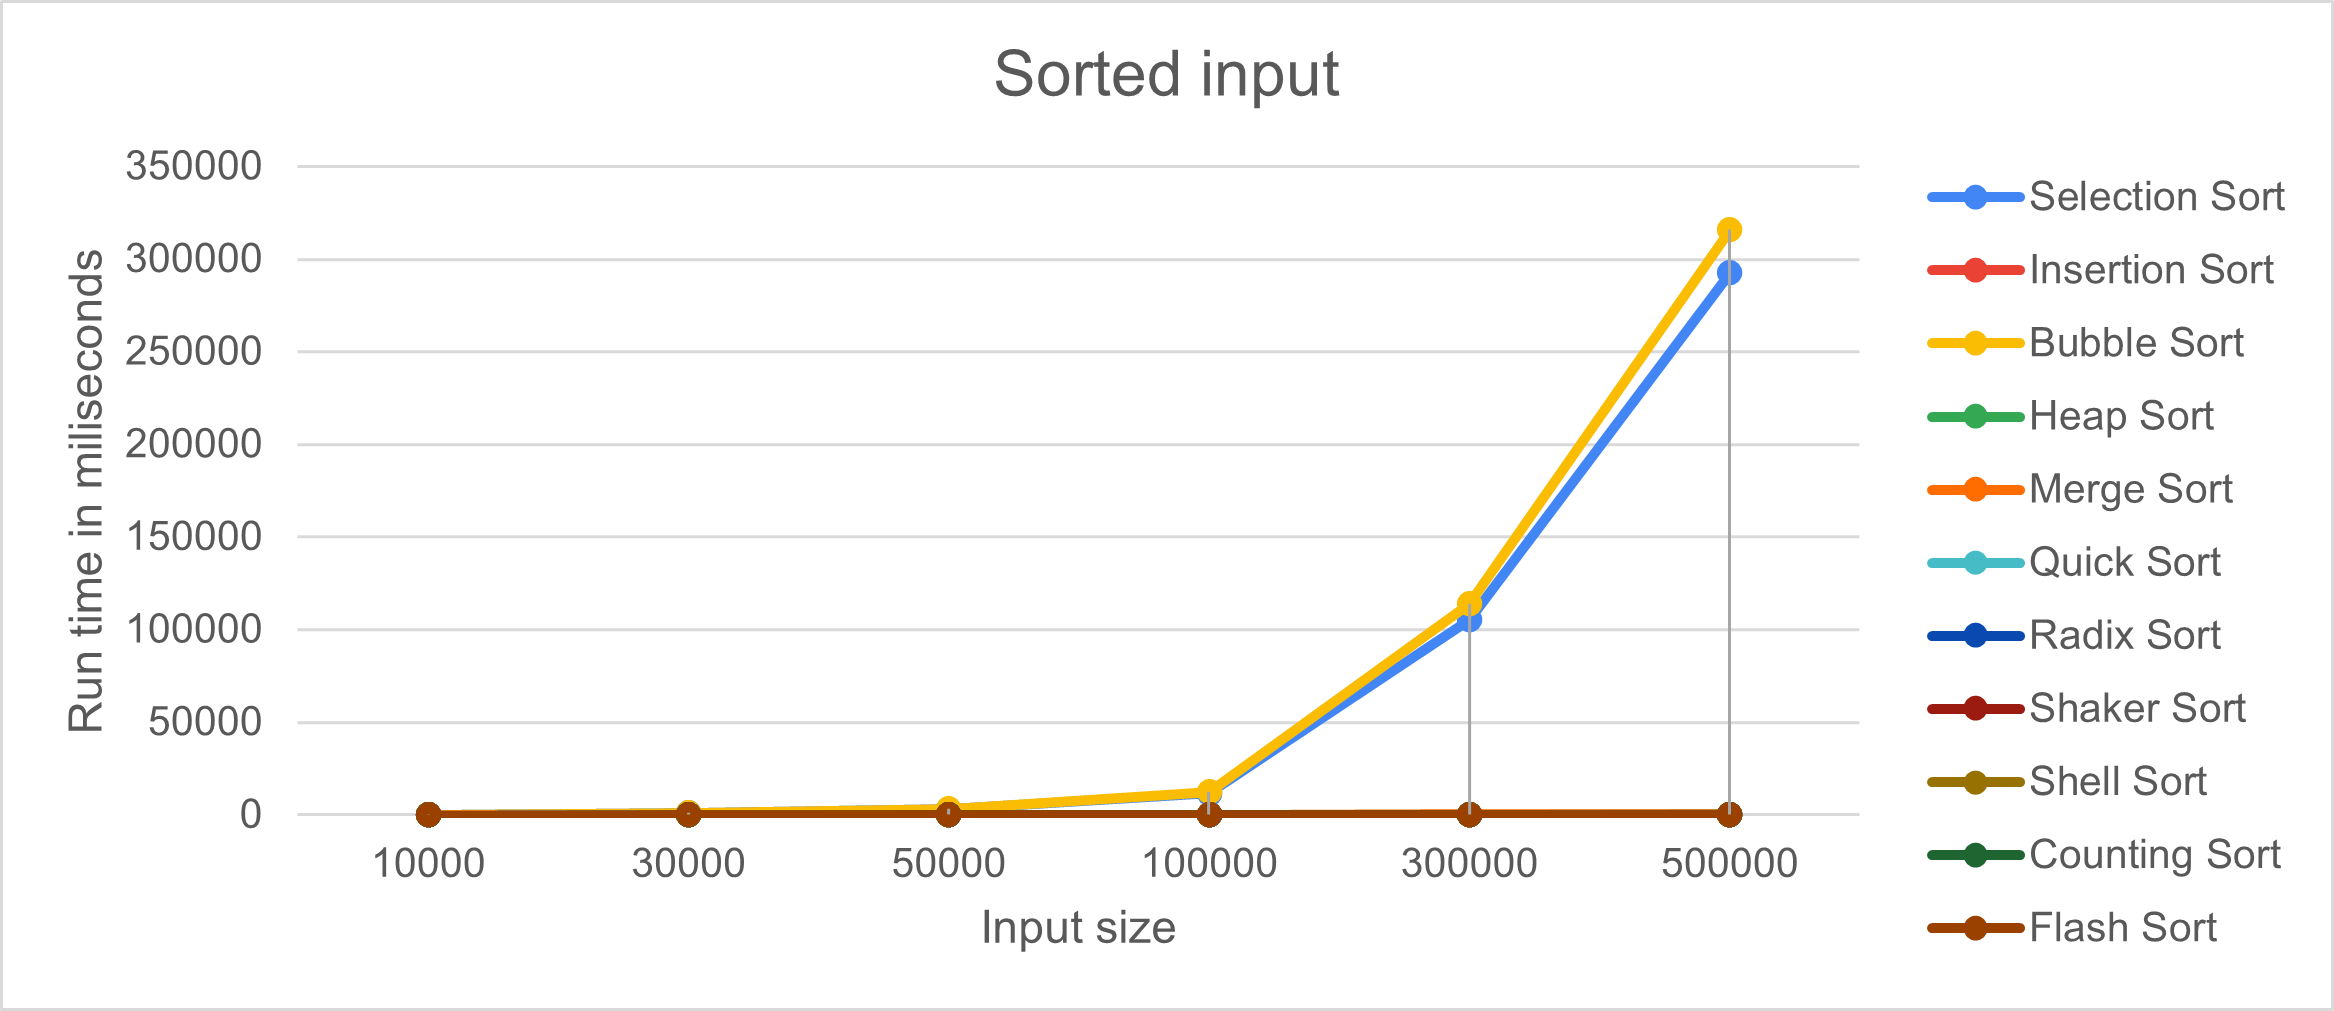
\includegraphics[scale = 0.8]{SortedLines.png}
\caption{ A line graph for visualizing the algorithms’ running times on sorted data.}
\centering
\end{figure}

\tab From what we can see, bubble sort and selection sort take the most amount of time out of all other algorithms when we gradually increases the size of the input data. The time it takes increase exponentially. This is due to the nature of these two sorting algorithms still trying to sort the input while the input itself is already sorted.

\begin{figure}[H]
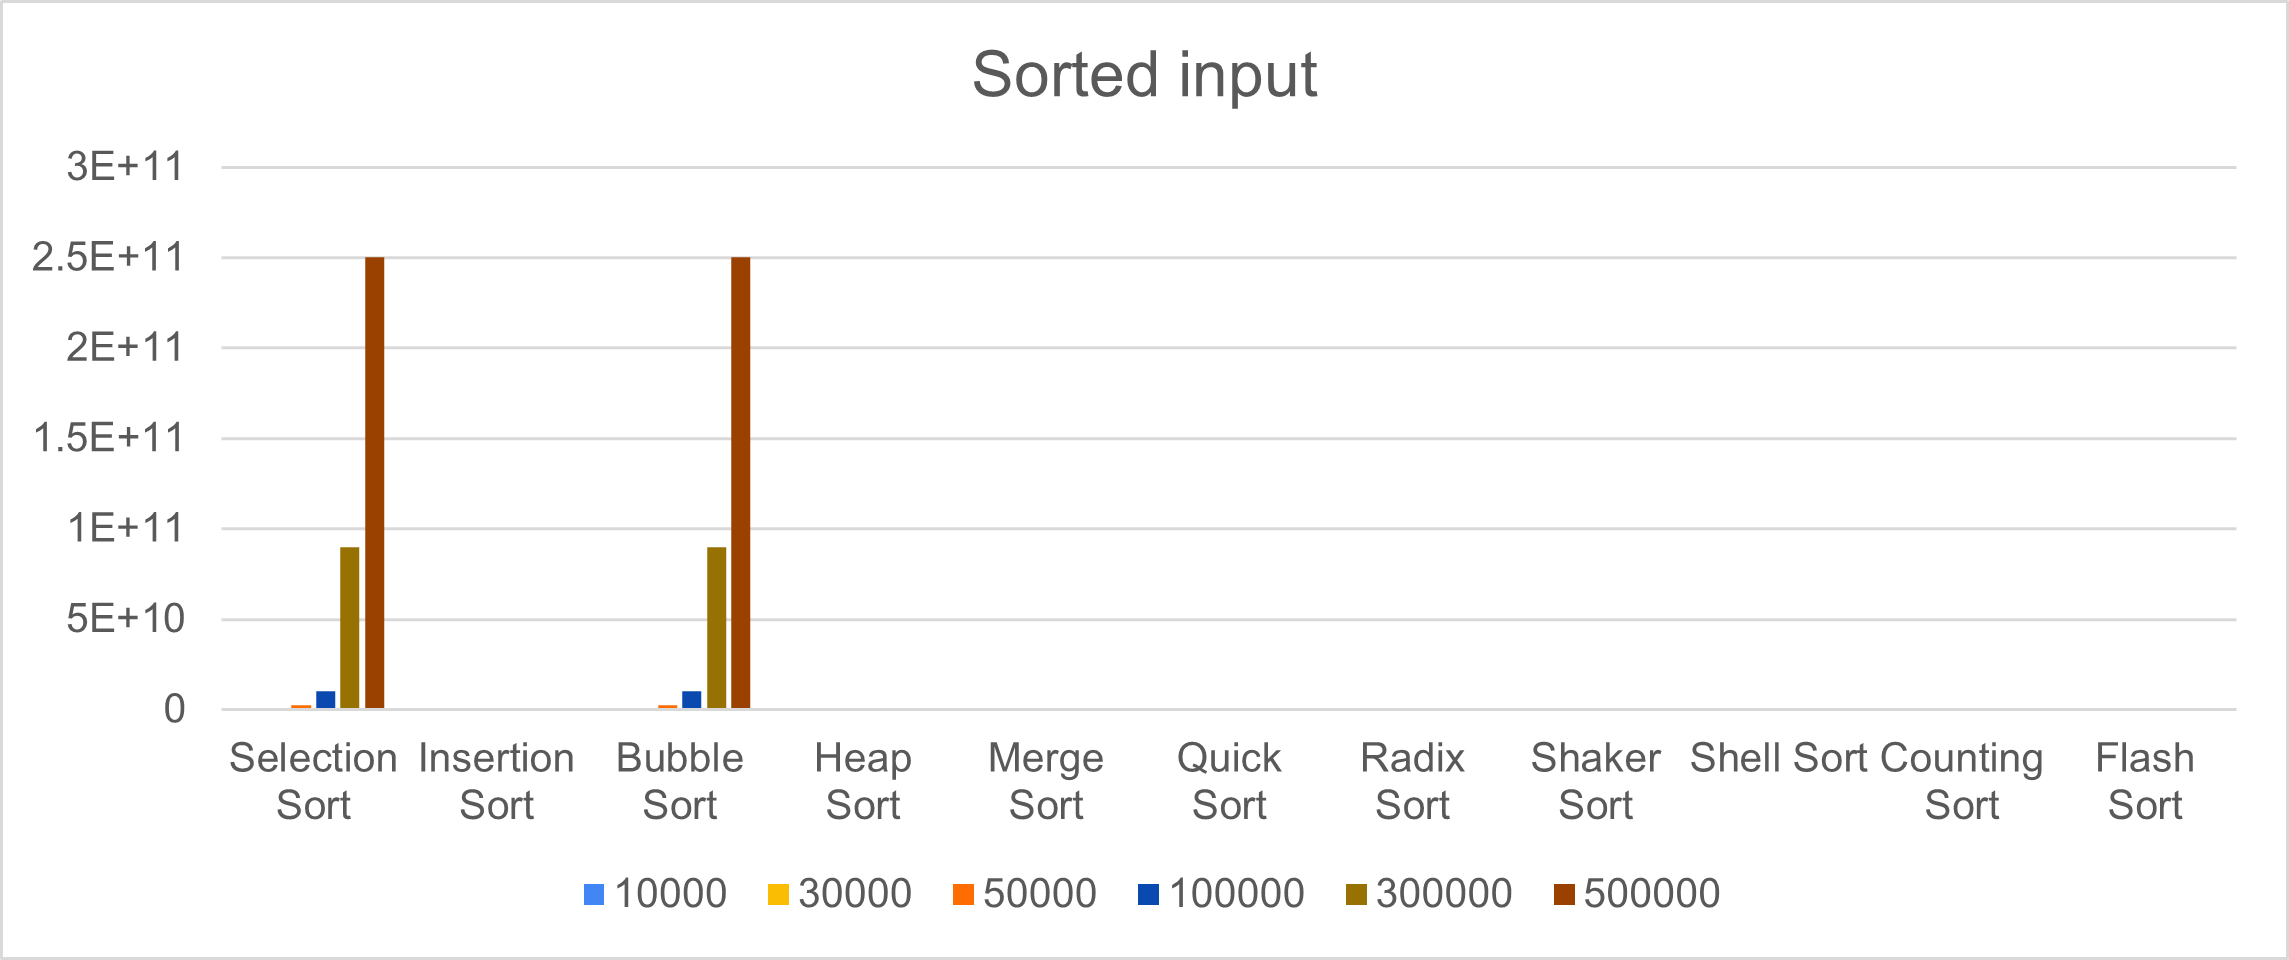
\includegraphics[scale = 0.8]{SortedBar.png}
\caption{A bar graph for visualizing the algorithms’ comparisons on sorted data.}
\centering
\end{figure}

We can see a familiar trend when comparing comparisons, bubble sort and selection sort still take the lead in the most amount of the comparisons. The reason for this is that bubble and selection are comparison-based sorting algorithms, but insertion sort is also comparison-based then why does it take very little comparisons. When the algorithm is already sorted, insertion sort doesn't need to move elements around very much.

\subsubsection{Nearly sorted data}
\begin{table}[H]
\begin{adjustbox}{width=\columnwidth,center}
\begin{tabular}{|l|rrrrrrrrrrrr|}
\hline
                  & \multicolumn{12}{c|}{Nearly sorted data}                                                                                                                                                                                                                                                                                                                                                                                           \\ \hline
Data size         & \multicolumn{2}{c|}{10000}                                          & \multicolumn{2}{c|}{30000}                                          & \multicolumn{2}{c|}{50000}                                          & \multicolumn{2}{c|}{100000}                                         & \multicolumn{2}{c|}{300000}                                          & \multicolumn{2}{c|}{500000}                                         \\ \hline
Resulting statics & \multicolumn{1}{l|}{Running time} & \multicolumn{1}{l|}{Comparison} & \multicolumn{1}{l|}{Running time} & \multicolumn{1}{l|}{Comparison} & \multicolumn{1}{l|}{Running time} & \multicolumn{1}{l|}{Comparison} & \multicolumn{1}{l|}{Running time} & \multicolumn{1}{l|}{Comparison} & \multicolumn{1}{l|}{Running time} & \multicolumn{1}{l|}{Comparison}  & \multicolumn{1}{l|}{Running time} & \multicolumn{1}{l|}{Comparison} \\ \hline
Selection Sort    & \multicolumn{1}{r|}{119}          & \multicolumn{1}{r|}{99999999}   & \multicolumn{1}{r|}{1072}         & \multicolumn{1}{r|}{899999999}  & \multicolumn{1}{r|}{2946}         & \multicolumn{1}{r|}{2499999999} & \multicolumn{1}{r|}{11668}        & \multicolumn{1}{r|}{9999999999} & \multicolumn{1}{r|}{105220}       & \multicolumn{1}{r|}{89999999999} & \multicolumn{1}{r|}{293361}       & 249999999999                    \\ \hline
Insertion Sort    & \multicolumn{1}{r|}{1}            & \multicolumn{1}{r|}{178607}     & \multicolumn{1}{r|}{1}            & \multicolumn{1}{r|}{403703}     & \multicolumn{1}{r|}{1}            & \multicolumn{1}{r|}{503547}     & \multicolumn{1}{r|}{1}            & \multicolumn{1}{r|}{448567}     & \multicolumn{1}{r|}{2}            & \multicolumn{1}{r|}{780479}      & \multicolumn{1}{r|}{2}            & 1090751                         \\ \hline
Bubble Sort       & \multicolumn{1}{r|}{128}          & \multicolumn{1}{r|}{99999999}   & \multicolumn{1}{r|}{1150}         & \multicolumn{1}{r|}{899999999}  & \multicolumn{1}{r|}{3177}         & \multicolumn{1}{r|}{2499999999} & \multicolumn{1}{r|}{12637}        & \multicolumn{1}{r|}{9999999999} & \multicolumn{1}{r|}{113604}       & \multicolumn{1}{r|}{89999999999} & \multicolumn{1}{r|}{314298}       & 249999999999                    \\ \hline
Heap Sort         & \multicolumn{1}{r|}{3}            & \multicolumn{1}{r|}{504035}     & \multicolumn{1}{r|}{9}            & \multicolumn{1}{r|}{1697754}    & \multicolumn{1}{r|}{16}           & \multicolumn{1}{r|}{2985884}    & \multicolumn{1}{r|}{34}           & \multicolumn{1}{r|}{6375400}    & \multicolumn{1}{r|}{122}          & \multicolumn{1}{r|}{21011315}    & \multicolumn{1}{r|}{208}          & 36433444                        \\ \hline
Merge Sort        & \multicolumn{1}{r|}{7}            & \multicolumn{1}{r|}{572353}     & \multicolumn{1}{r|}{20}           & \multicolumn{1}{r|}{1878876}    & \multicolumn{1}{r|}{34}           & \multicolumn{1}{r|}{3167875}    & \multicolumn{1}{r|}{69}           & \multicolumn{1}{r|}{6411694}    & \multicolumn{1}{r|}{209}          & \multicolumn{1}{r|}{20554939}    & \multicolumn{1}{r|}{358}          & 35631995                        \\ \hline
Quick Sort        & \multicolumn{1}{r|}{1}            & \multicolumn{1}{r|}{163613}     & \multicolumn{1}{r|}{2}            & \multicolumn{1}{r|}{537229}     & \multicolumn{1}{r|}{3}            & \multicolumn{1}{r|}{934461}     & \multicolumn{1}{r|}{6}            & \multicolumn{1}{r|}{1968925}    & \multicolumn{1}{r|}{22}           & \multicolumn{1}{r|}{6375709}     & \multicolumn{1}{r|}{36}           & 10975709                        \\ \hline
Radix Sort        & \multicolumn{1}{r|}{2}            & \multicolumn{1}{r|}{140038}     & \multicolumn{1}{r|}{7}            & \multicolumn{1}{r|}{510048}     & \multicolumn{1}{r|}{13}           & \multicolumn{1}{r|}{850048}     & \multicolumn{1}{r|}{27}           & \multicolumn{1}{r|}{1700048}    & \multicolumn{1}{r|}{92}           & \multicolumn{1}{r|}{6000058}     & \multicolumn{1}{r|}{157}          & 10000058                        \\ \hline
Shaker Sort       & \multicolumn{1}{r|}{1}            & \multicolumn{1}{r|}{212133}     & \multicolumn{1}{r|}{2}            & \multicolumn{1}{r|}{461240}     & \multicolumn{1}{r|}{2}            & \multicolumn{1}{r|}{680143}     & \multicolumn{1}{r|}{3}            & \multicolumn{1}{r|}{916171}     & \multicolumn{1}{r|}{6}            & \multicolumn{1}{r|}{1555945}     & \multicolumn{1}{r|}{6}            & 2291317                         \\ \hline
Shell Sort        & \multicolumn{1}{r|}{1}            & \multicolumn{1}{r|}{137996}     & \multicolumn{1}{r|}{2}            & \multicolumn{1}{r|}{468005}     & \multicolumn{1}{r|}{3}            & \multicolumn{1}{r|}{768917}     & \multicolumn{1}{r|}{5}            & \multicolumn{1}{r|}{1581068}    & \multicolumn{1}{r|}{15}           & \multicolumn{1}{r|}{5186402}     & \multicolumn{1}{r|}{25}           & 8564843                         \\ \hline
Counting Sort     & \multicolumn{1}{r|}{0}            & \multicolumn{1}{r|}{89995}      & \multicolumn{1}{r|}{1}            & \multicolumn{1}{r|}{269995}     & \multicolumn{1}{r|}{1}            & \multicolumn{1}{r|}{449995}     & \multicolumn{1}{r|}{2}            & \multicolumn{1}{r|}{899995}     & \multicolumn{1}{r|}{9}            & \multicolumn{1}{r|}{2699995}     & \multicolumn{1}{r|}{14}           & 4499995                         \\ \hline
Flash Sort        & \multicolumn{1}{r|}{0}            & \multicolumn{1}{r|}{20983}      & \multicolumn{1}{r|}{1}            & \multicolumn{1}{r|}{62989}      & \multicolumn{1}{r|}{2}            & \multicolumn{1}{r|}{104985}     & \multicolumn{1}{r|}{5}            & \multicolumn{1}{r|}{209985}     & \multicolumn{1}{r|}{13}           & \multicolumn{1}{r|}{629987}      & \multicolumn{1}{r|}{22}           & 1049987                         \\ \hline
\end{tabular}
\end{adjustbox}
\end{table}
\begin{figure}[H]
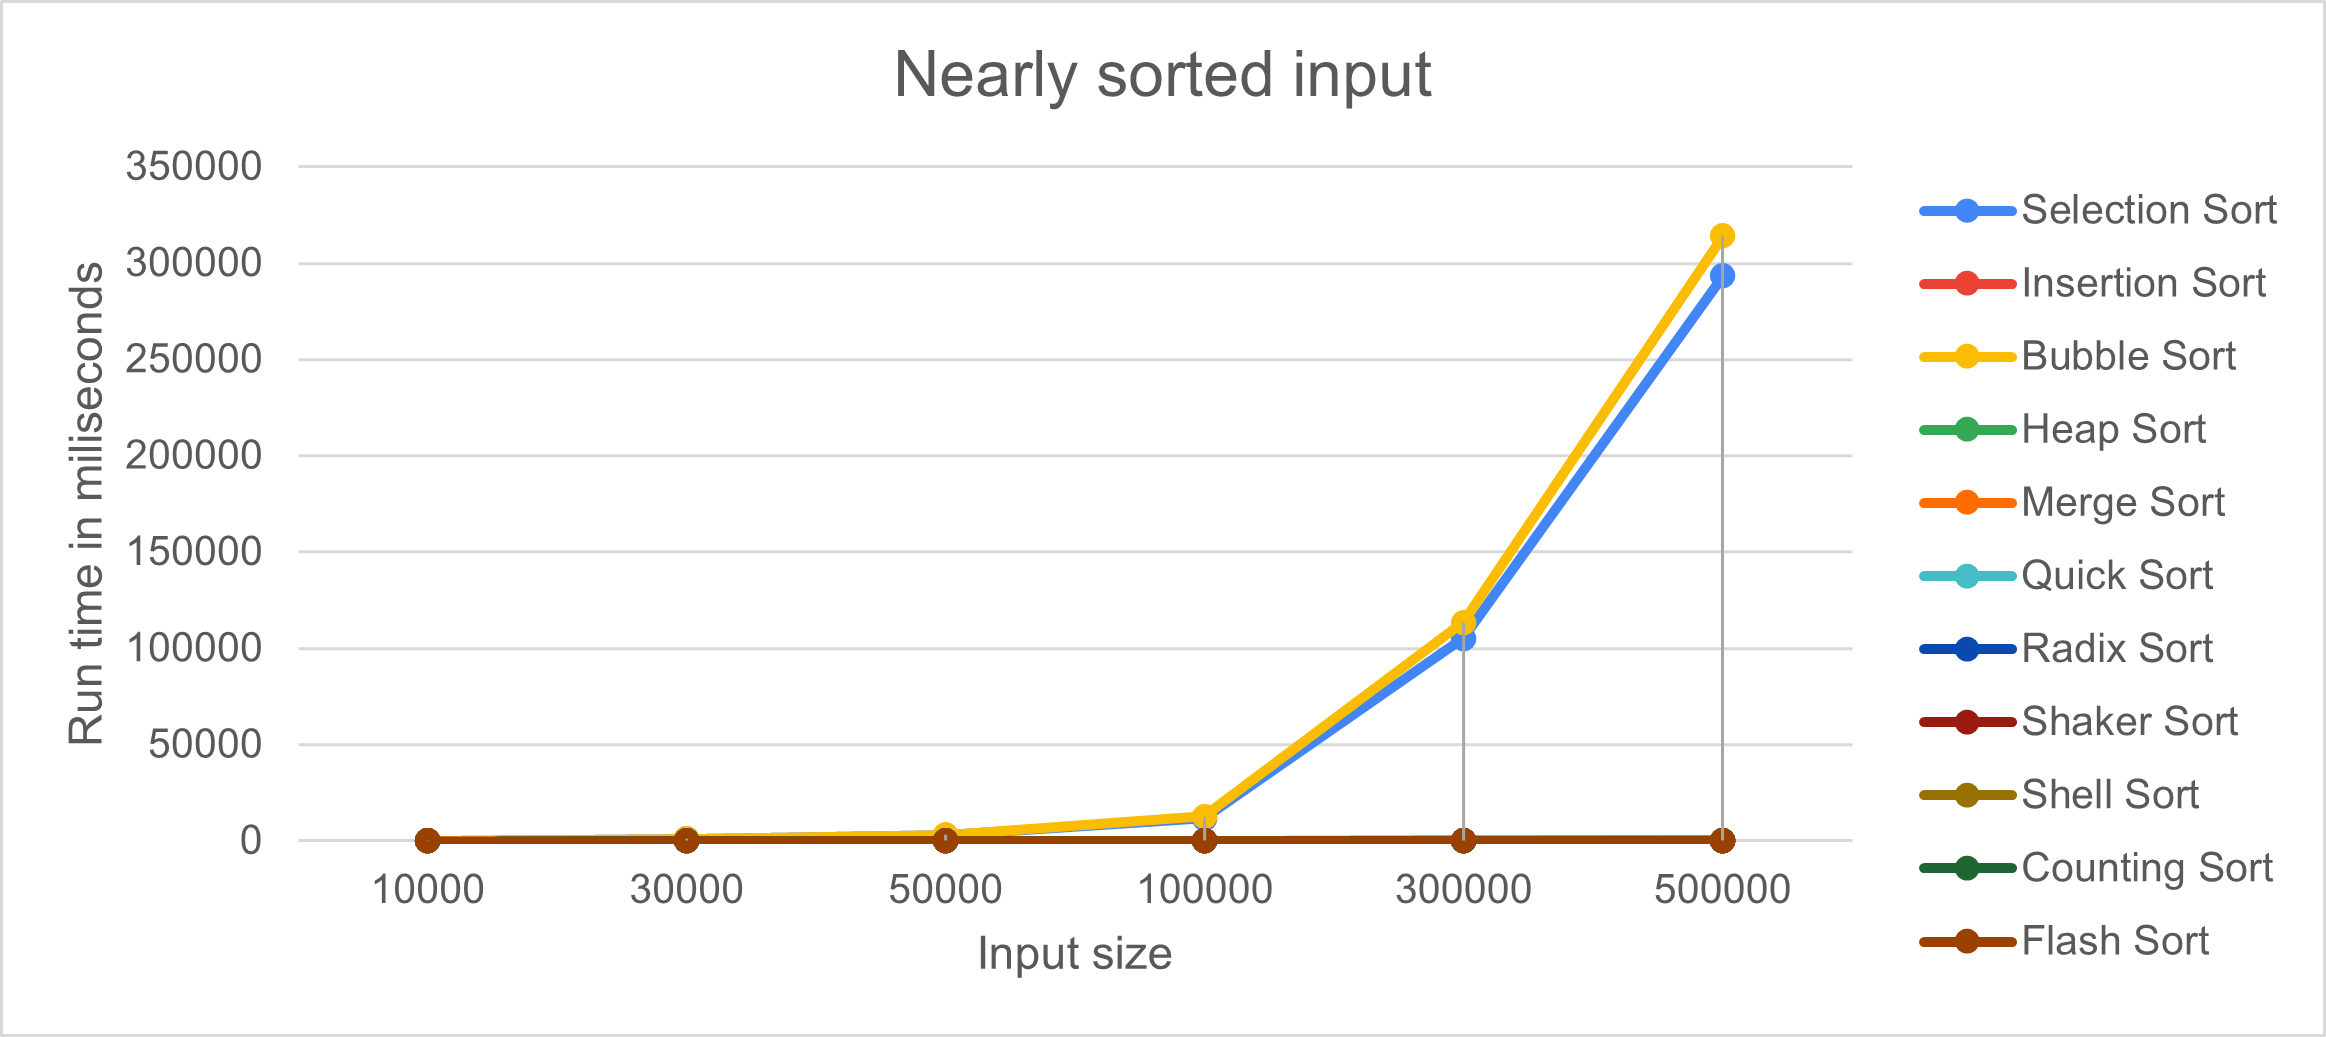
\includegraphics[scale = 0.8]{NSortedLines.png}
\caption{ A line graph for visualizing the algorithms’ running times on nearly sorted data.}
\centering
\end{figure}

\tab Nearly sorted data  is almost the same as sorted data with a little change is that insertion sort needs a bit more comparison due to the nature of the nearly sorted data.

\begin{figure}[H]
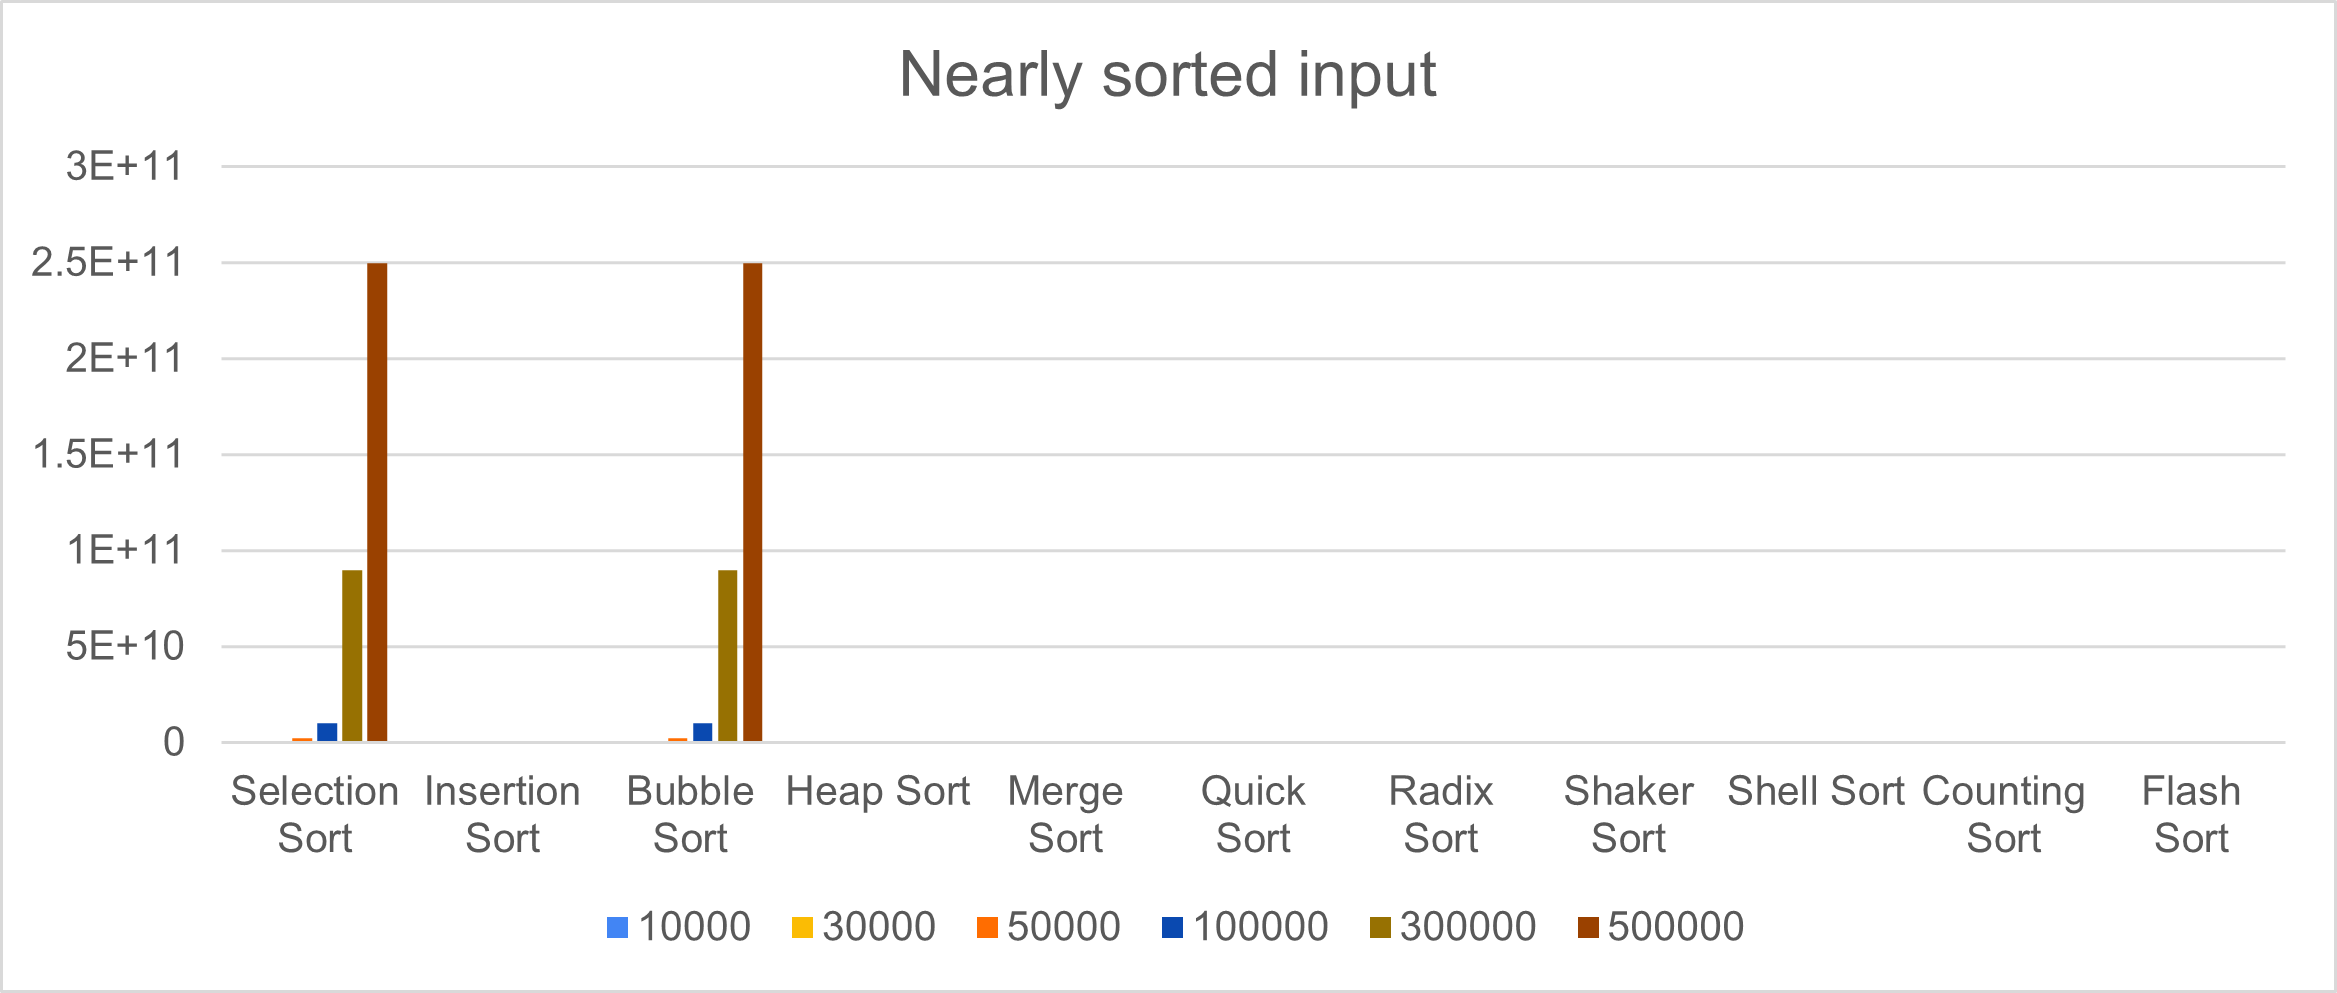
\includegraphics[scale = 0.8]{NSortedBar.png}
\caption{A bar graph for visualizing the algorithms’ comparisons on nearly sorted data.}
\centering
\end{figure}

Although the graph does not portray the changes in insertion sort, looking at the table provided, we can see that there is a difference comparing sorted and unsorted data from insertion sort.

\subsubsection{Reversed sorted data}

\begin{table}[H]
\begin{adjustbox}{width=\columnwidth,center}
\begin{tabular}{|l|rrrrrrrrrrrr|}
\hline
                                   & \multicolumn{12}{c|}{reversedd sorted data}                                                                                                                                                                                                                                                                                                                                                                                           \\ \hline
Data size                          & \multicolumn{2}{c|}{10000}                                          & \multicolumn{2}{c|}{30000}                                          & \multicolumn{2}{c|}{50000}                                          & \multicolumn{2}{c|}{100000}                                          & \multicolumn{2}{c|}{300000}                                          & \multicolumn{2}{c|}{500000}                                         \\ \hline
Resulting statics                  & \multicolumn{1}{l|}{Running time} & \multicolumn{1}{l|}{Comparison} & \multicolumn{1}{l|}{Running time} & \multicolumn{1}{l|}{Comparison} & \multicolumn{1}{l|}{Running time} & \multicolumn{1}{l|}{Comparison} & \multicolumn{1}{l|}{Running time} & \multicolumn{1}{l|}{Comparison}  & \multicolumn{1}{l|}{Running time} & \multicolumn{1}{l|}{Comparison}  & \multicolumn{1}{l|}{Running time} & \multicolumn{1}{l|}{Comparison} \\ \hline
Selection Sort                     & \multicolumn{1}{r|}{125}          & \multicolumn{1}{r|}{99999999}   & \multicolumn{1}{r|}{1086}         & \multicolumn{1}{r|}{899999999}  & \multicolumn{1}{r|}{3062}         & \multicolumn{1}{r|}{2499999999} & \multicolumn{1}{r|}{12161}        & \multicolumn{1}{r|}{9999999999}  & \multicolumn{1}{r|}{108994}       & \multicolumn{1}{r|}{89999999999} & \multicolumn{1}{r|}{302903}       & 249999999999                    \\ \hline
Insertion Sort                     & \multicolumn{1}{r|}{136}          & \multicolumn{1}{r|}{99999999}   & \multicolumn{1}{r|}{1230}         & \multicolumn{1}{r|}{899999999}  & \multicolumn{1}{r|}{3387}         & \multicolumn{1}{r|}{2499999999} & \multicolumn{1}{r|}{15163}        & \multicolumn{1}{r|}{9999999999}  & \multicolumn{1}{r|}{168939}       & \multicolumn{1}{r|}{89999999999} & \multicolumn{1}{r|}{276609}       & 249999999999                    \\ \hline
Bubble Sort                        & \multicolumn{1}{r|}{353}          & \multicolumn{1}{r|}{99999999}   & \multicolumn{1}{r|}{1799}         & \multicolumn{1}{r|}{899999999}  & \multicolumn{1}{r|}{5028}         & \multicolumn{1}{r|}{2499999999} & \multicolumn{1}{r|}{20089}        & \multicolumn{1}{r|}{9999999999}  & \multicolumn{1}{r|}{181257}       & \multicolumn{1}{r|}{89999999999} & \multicolumn{1}{r|}{741422}       & 249999999999                    \\ \hline
Heap Sort                          & \multicolumn{1}{r|}{3}            & \multicolumn{1}{r|}{468401}     & \multicolumn{1}{r|}{9}            & \multicolumn{1}{r|}{1596468}    & \multicolumn{1}{r|}{15}           & \multicolumn{1}{r|}{2807198}    & \multicolumn{1}{r|}{32}           & \multicolumn{1}{r|}{6003393}     & \multicolumn{1}{r|}{111}          & \multicolumn{1}{r|}{19931637}    & \multicolumn{1}{r|}{190}          & 34706560                        \\ \hline
Merge Sort                         & \multicolumn{1}{r|}{7}            & \multicolumn{1}{r|}{534251}     & \multicolumn{1}{r|}{20}           & \multicolumn{1}{r|}{1757643}    & \multicolumn{1}{r|}{35}           & \multicolumn{1}{r|}{3074779}    & \multicolumn{1}{r|}{70}           & \multicolumn{1}{r|}{6499563}     & \multicolumn{1}{r|}{212}          & \multicolumn{1}{r|}{21143211}    & \multicolumn{1}{r|}{362}          & 36301067                        \\ \hline
Quick Sort & \multicolumn{1}{r|}{1}            & \multicolumn{1}{r|}{163612}     & \multicolumn{1}{r|}{2}            & \multicolumn{1}{r|}{537228}     & \multicolumn{1}{r|}{4}            & \multicolumn{1}{r|}{934460}     & \multicolumn{1}{r|}{6}            & \multicolumn{1}{r|}{1968924}     & \multicolumn{1}{r|}{20}           & \multicolumn{1}{r|}{6375708}     & \multicolumn{1}{r|}{35}           & 10975708                        \\ \hline
Radix Sort                         & \multicolumn{1}{r|}{2}            & \multicolumn{1}{r|}{140038}     & \multicolumn{1}{r|}{7}            & \multicolumn{1}{r|}{510048}     & \multicolumn{1}{r|}{13}           & \multicolumn{1}{r|}{850048}     & \multicolumn{1}{r|}{26}           & \multicolumn{1}{r|}{1700048}     & \multicolumn{1}{r|}{94}           & \multicolumn{1}{r|}{6000058}     & \multicolumn{1}{r|}{156}          & 10000058                        \\ \hline
Shaker Sort                        & \multicolumn{1}{r|}{276}          & \multicolumn{1}{r|}{100004999}  & \multicolumn{1}{r|}{1409}         & \multicolumn{1}{r|}{900014999}  & \multicolumn{1}{r|}{3937}         & \multicolumn{1}{r|}{2500024999} & \multicolumn{1}{r|}{15731}        & \multicolumn{1}{r|}{10000049999} & \multicolumn{1}{r|}{141924}       & \multicolumn{1}{r|}{90000149999} & \multicolumn{1}{r|}{580533}       & 250000249999                    \\ \hline
Shell Sort                         & \multicolumn{1}{r|}{1}            & \multicolumn{1}{r|}{182578}     & \multicolumn{1}{r|}{4}            & \multicolumn{1}{r|}{597013}     & \multicolumn{1}{r|}{7}            & \multicolumn{1}{r|}{1097301}    & \multicolumn{1}{r|}{16}           & \multicolumn{1}{r|}{2344582}     & \multicolumn{1}{r|}{49}           & \multicolumn{1}{r|}{7600906}     & \multicolumn{1}{r|}{87}           & 12928777                        \\ \hline
Counting Sort                      & \multicolumn{1}{r|}{0}            & \multicolumn{1}{r|}{89995}      & \multicolumn{1}{r|}{1}            & \multicolumn{1}{r|}{269995}     & \multicolumn{1}{r|}{1}            & \multicolumn{1}{r|}{449995}     & \multicolumn{1}{r|}{3}            & \multicolumn{1}{r|}{899995}      & \multicolumn{1}{r|}{7}            & \multicolumn{1}{r|}{2699995}     & \multicolumn{1}{r|}{12}           & 4499995                         \\ \hline
Flash Sort                         & \multicolumn{1}{r|}{0}            & \multicolumn{1}{r|}{17503}      & \multicolumn{1}{r|}{1}            & \multicolumn{1}{r|}{52503}      & \multicolumn{1}{r|}{2}            & \multicolumn{1}{r|}{87503}      & \multicolumn{1}{r|}{4}            & \multicolumn{1}{r|}{175003}      & \multicolumn{1}{r|}{13}           & \multicolumn{1}{r|}{525003}      & \multicolumn{1}{r|}{21}           & 875003                          \\ \hline
\end{tabular}
\end{adjustbox}
\end{table}

\begin{figure}[H]
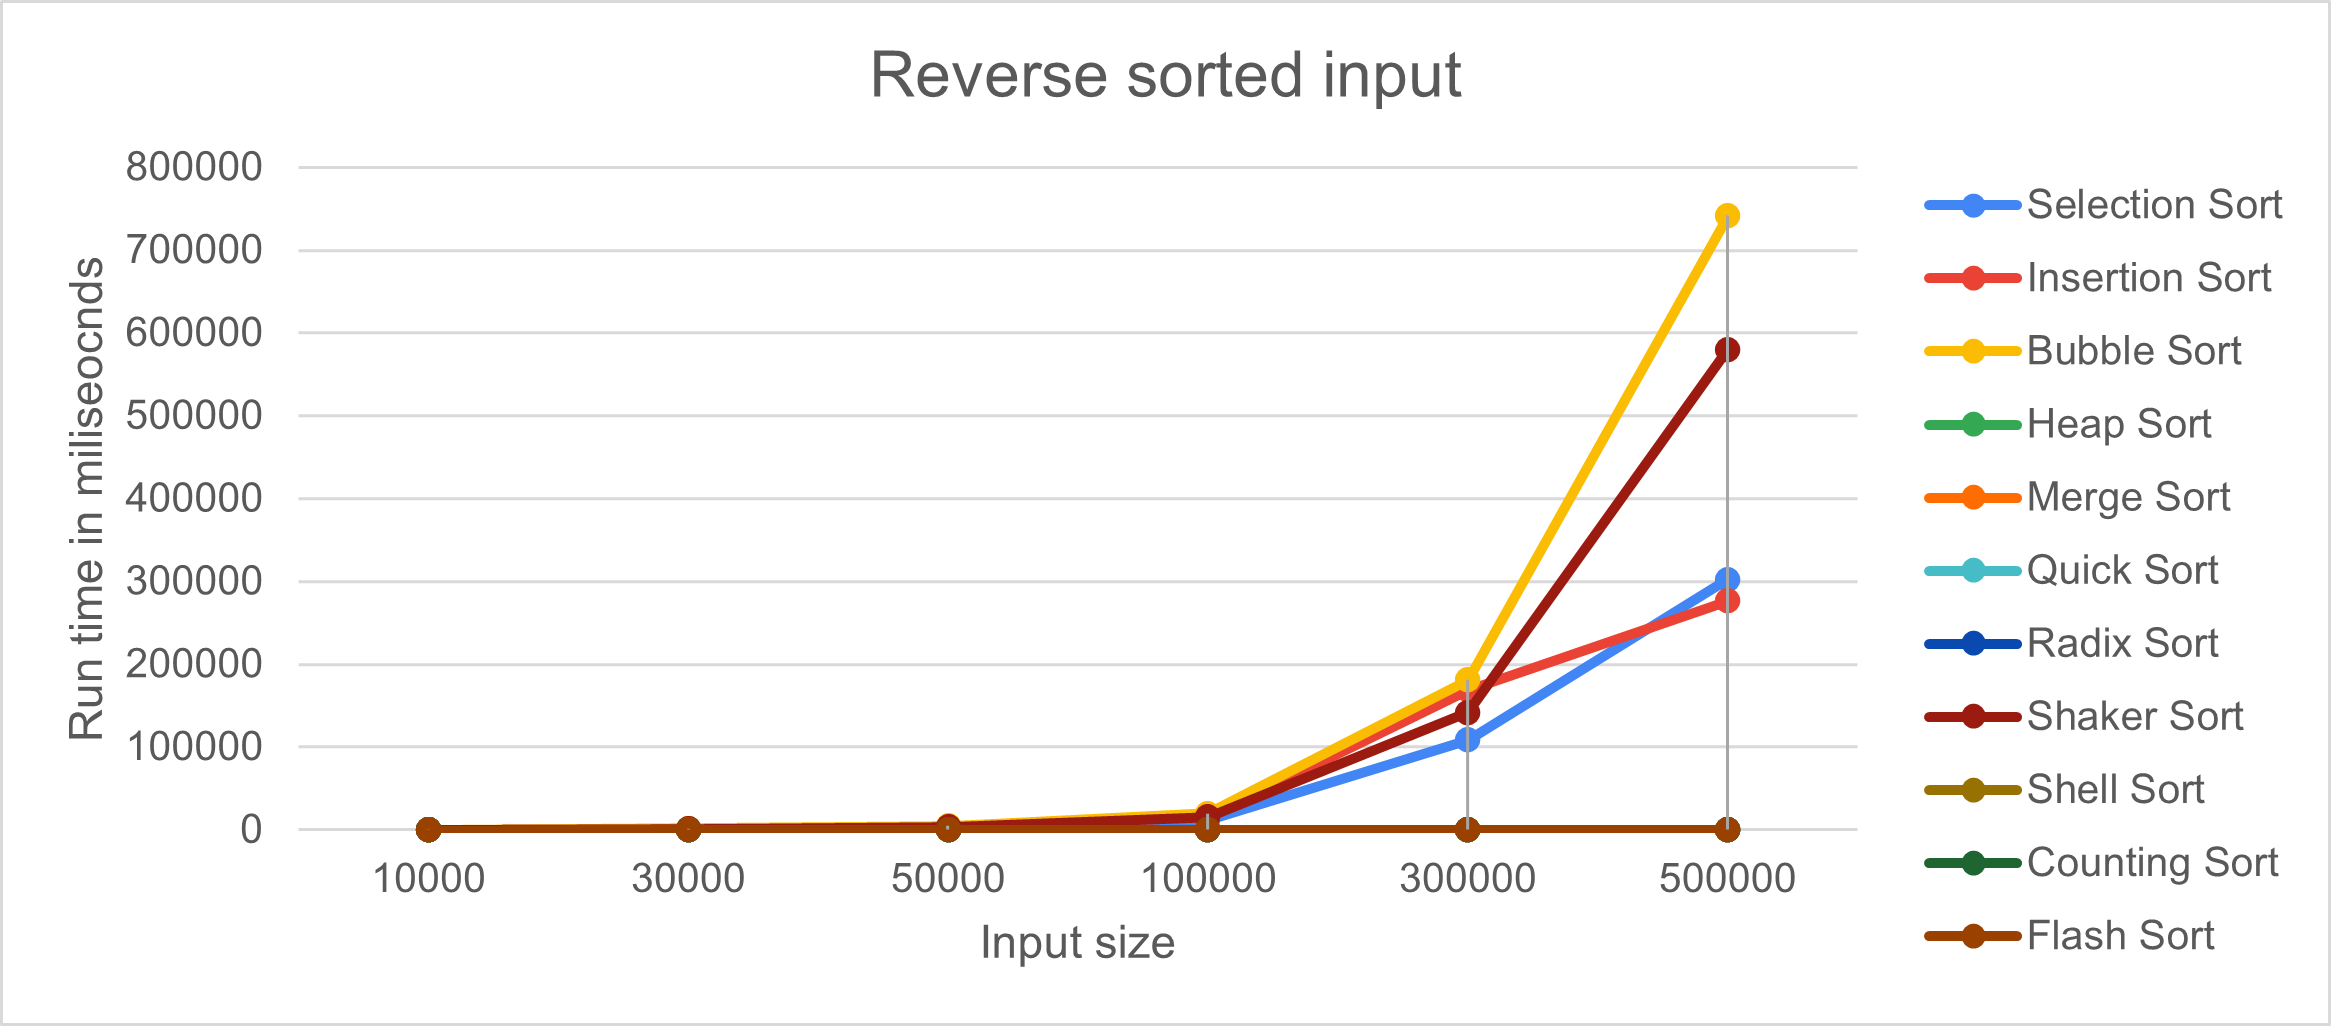
\includegraphics[scale = 0.8]{!SortedLines.png}
\caption{ A line graph for visualizing the algorithms’ running times reversed on sorted data.}
\centering
\end{figure}

\tab Looking at the line graph, we can see a lot of changes from the previous two graph. Bubble sort is still the longest one. However shaker sort now takes the second place from selection sort. Most notably, selection sort is now almost as fast merge sort. We can understand why shaker sort takes a sudden change, if every element is at a position that differs by at most k (k ≥ 1) from the position it is going to end up in, the complexity of cocktail shaker sort becomes ($O(kn)$).

\begin{figure}[H]
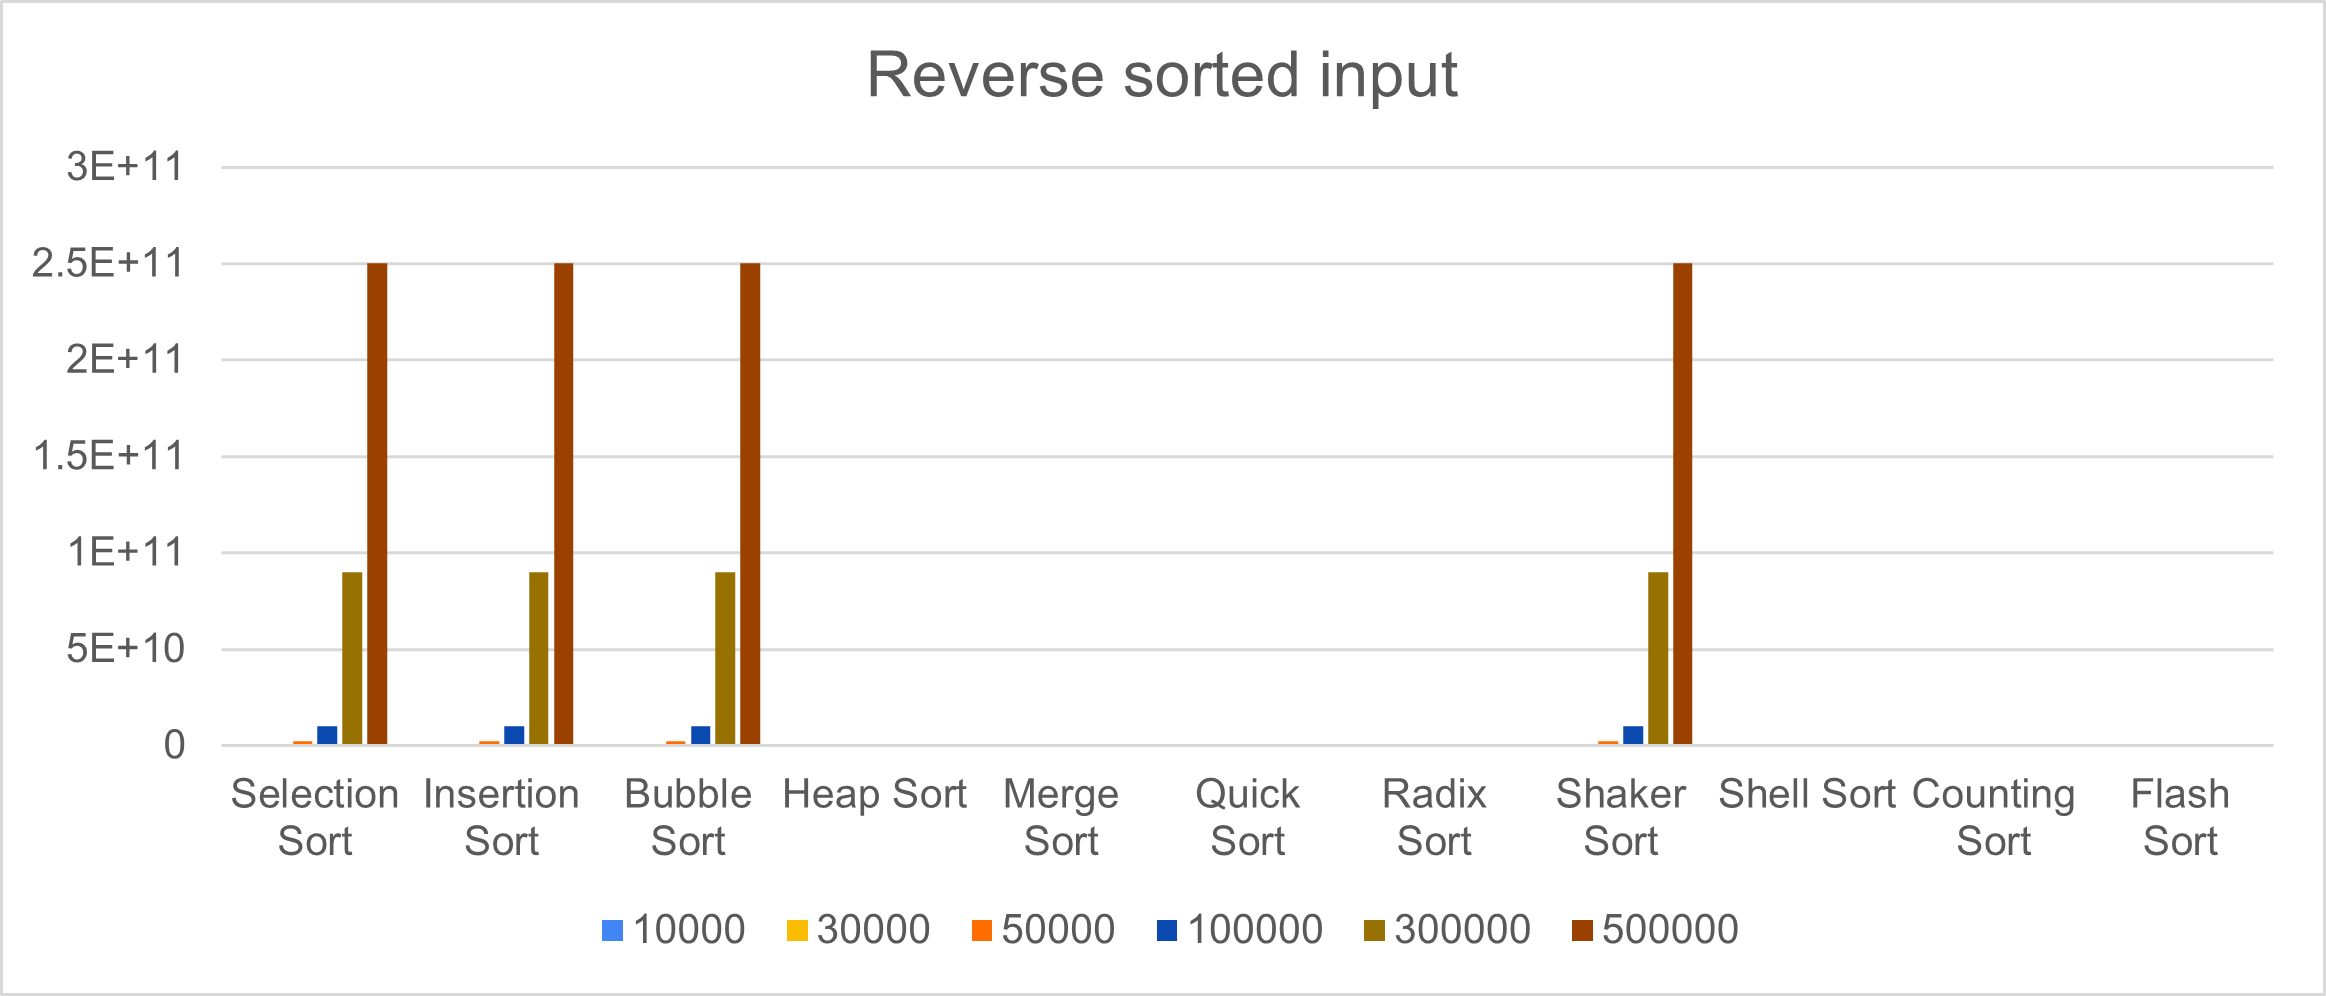
\includegraphics[scale = 0.8]{!SortedBar.png}
\caption{A bar graph for visualizing the algorithms’ comparisons on reversed sorted data.}
\centering
\end{figure}

Here we can see insertion and shaker sort in their worst-case scenario with a high number of comparisons.

\subsubsection{Randomized data}
\begin{table}[H]
\begin{adjustbox}{width=\columnwidth,center}
\begin{tabular}{|l|rrrrrrrrrrrr|}
\hline
                                   & \multicolumn{12}{c|}{Randomized data}                                                                                                                                                                                                                                                                                                                                                                                              \\ \hline
Data size                          & \multicolumn{2}{c|}{10000}                                          & \multicolumn{2}{c|}{30000}                                          & \multicolumn{2}{c|}{50000}                                          & \multicolumn{2}{c|}{100000}                                         & \multicolumn{2}{c|}{300000}                                          & \multicolumn{2}{c|}{500000}                                         \\ \hline
Resulting statics                  & \multicolumn{1}{l|}{Running time} & \multicolumn{1}{l|}{Comparison} & \multicolumn{1}{l|}{Running time} & \multicolumn{1}{l|}{Comparison} & \multicolumn{1}{l|}{Running time} & \multicolumn{1}{l|}{Comparison} & \multicolumn{1}{l|}{Running time} & \multicolumn{1}{l|}{Comparison} & \multicolumn{1}{l|}{Running time} & \multicolumn{1}{l|}{Comparison}  & \multicolumn{1}{l|}{Running time} & \multicolumn{1}{l|}{Comparison} \\ \hline
Selection Sort                     & \multicolumn{1}{r|}{121}          & \multicolumn{1}{r|}{99999999}   & \multicolumn{1}{r|}{1064}         & \multicolumn{1}{r|}{899999999}  & \multicolumn{1}{r|}{2948}         & \multicolumn{1}{r|}{2499999999} & \multicolumn{1}{r|}{11740}        & \multicolumn{1}{r|}{9999999999} & \multicolumn{1}{r|}{105523}       & \multicolumn{1}{r|}{89999999999} & \multicolumn{1}{r|}{292372}       & 249999999999                    \\ \hline
Insertion Sort                     & \multicolumn{1}{r|}{66}           & \multicolumn{1}{r|}{49836639}   & \multicolumn{1}{r|}{607}          & \multicolumn{1}{r|}{448748189}  & \multicolumn{1}{r|}{1697}         & \multicolumn{1}{r|}{1248310235} & \multicolumn{1}{r|}{6763}         & \multicolumn{1}{r|}{4986397423} & \multicolumn{1}{r|}{95985}        & \multicolumn{1}{r|}{45016486265} & \multicolumn{1}{r|}{337577}       & 125071744873                    \\ \hline
Bubble Sort                        & \multicolumn{1}{r|}{293}          & \multicolumn{1}{r|}{99999999}   & \multicolumn{1}{r|}{2165}         & \multicolumn{1}{r|}{899999999}  & \multicolumn{1}{r|}{6298}         & \multicolumn{1}{r|}{2499999999} & \multicolumn{1}{r|}{26354}        & \multicolumn{1}{r|}{9999999999} & \multicolumn{1}{r|}{224869}       & \multicolumn{1}{r|}{89999999999} & \multicolumn{1}{r|}{793164}       & 249999999999                    \\ \hline
Heap Sort                          & \multicolumn{1}{r|}{3}            & \multicolumn{1}{r|}{485564}     & \multicolumn{1}{r|}{10}           & \multicolumn{1}{r|}{1647028}    & \multicolumn{1}{r|}{18}           & \multicolumn{1}{r|}{2894853}    & \multicolumn{1}{r|}{37}           & \multicolumn{1}{r|}{6189279}    & \multicolumn{1}{r|}{124}          & \multicolumn{1}{r|}{20451193}    & \multicolumn{1}{r|}{217}          & 35542359                        \\ \hline
Merge Sort                         & \multicolumn{1}{r|}{7}            & \multicolumn{1}{r|}{734487}     & \multicolumn{1}{r|}{23}           & \multicolumn{1}{r|}{2465192}    & \multicolumn{1}{r|}{38}           & \multicolumn{1}{r|}{4312281}    & \multicolumn{1}{r|}{76}           & \multicolumn{1}{r|}{9173712}    & \multicolumn{1}{r|}{231}          & \multicolumn{1}{r|}{30129475}    & \multicolumn{1}{r|}{397}          & 52260910                        \\ \hline
Quick Sort & \multicolumn{1}{r|}{2}            & \multicolumn{1}{r|}{203030}     & \multicolumn{1}{r|}{4}            & \multicolumn{1}{r|}{692944}     & \multicolumn{1}{r|}{7}            & \multicolumn{1}{r|}{1213732}    & \multicolumn{1}{r|}{14}           & \multicolumn{1}{r|}{2473158}    & \multicolumn{1}{r|}{42}           & \multicolumn{1}{r|}{7807295}     & \multicolumn{1}{r|}{71}           & 13352871                        \\ \hline
Radix Sort                         & \multicolumn{1}{r|}{2}            & \multicolumn{1}{r|}{140038}     & \multicolumn{1}{r|}{7}            & \multicolumn{1}{r|}{510048}     & \multicolumn{1}{r|}{13}           & \multicolumn{1}{r|}{850048}     & \multicolumn{1}{r|}{25}           & \multicolumn{1}{r|}{1700048}    & \multicolumn{1}{r|}{74}           & \multicolumn{1}{r|}{6000058}     & \multicolumn{1}{r|}{122}          & 8500048                         \\ \hline
Shaker Sort                        & \multicolumn{1}{r|}{229}          & \multicolumn{1}{r|}{67132541}   & \multicolumn{1}{r|}{1695}         & \multicolumn{1}{r|}{597243042}  & \multicolumn{1}{r|}{4931}         & \multicolumn{1}{r|}{1662711596} & \multicolumn{1}{r|}{20635}        & \multicolumn{1}{r|}{6676026886} & \multicolumn{1}{r|}{176082}       & \multicolumn{1}{r|}{60045803655} & \multicolumn{1}{r|}{621047}       & 166766760719                    \\ \hline
Shell Sort                         & \multicolumn{1}{r|}{3}            & \multicolumn{1}{r|}{270047}     & \multicolumn{1}{r|}{11}           & \multicolumn{1}{r|}{980977}     & \multicolumn{1}{r|}{22}           & \multicolumn{1}{r|}{1843153}    & \multicolumn{1}{r|}{53}           & \multicolumn{1}{r|}{4310589}    & \multicolumn{1}{r|}{186}          & \multicolumn{1}{r|}{14978000}    & \multicolumn{1}{r|}{329}          & 26869564                        \\ \hline
Counting Sort                      & \multicolumn{1}{r|}{0}            & \multicolumn{1}{r|}{89993}      & \multicolumn{1}{r|}{0}            & \multicolumn{1}{r|}{269995}     & \multicolumn{1}{r|}{1}            & \multicolumn{1}{r|}{415525}     & \multicolumn{1}{r|}{2}            & \multicolumn{1}{r|}{765531}     & \multicolumn{1}{r|}{7}            & \multicolumn{1}{r|}{2165531}     & \multicolumn{1}{r|}{11}           & 3565531                         \\ \hline
Flash Sort                         & \multicolumn{1}{r|}{0}            & \multicolumn{1}{r|}{16661}      & \multicolumn{1}{r|}{1}            & \multicolumn{1}{r|}{51305}      & \multicolumn{1}{r|}{3}            & \multicolumn{1}{r|}{74375}      & \multicolumn{1}{r|}{5}            & \multicolumn{1}{r|}{99999}      & \multicolumn{1}{r|}{17}           & \multicolumn{1}{r|}{299999}      & \multicolumn{1}{r|}{28}           & 499999                          \\ \hline
\end{tabular}
\end{adjustbox}
\end{table}


\begin{figure}[H]
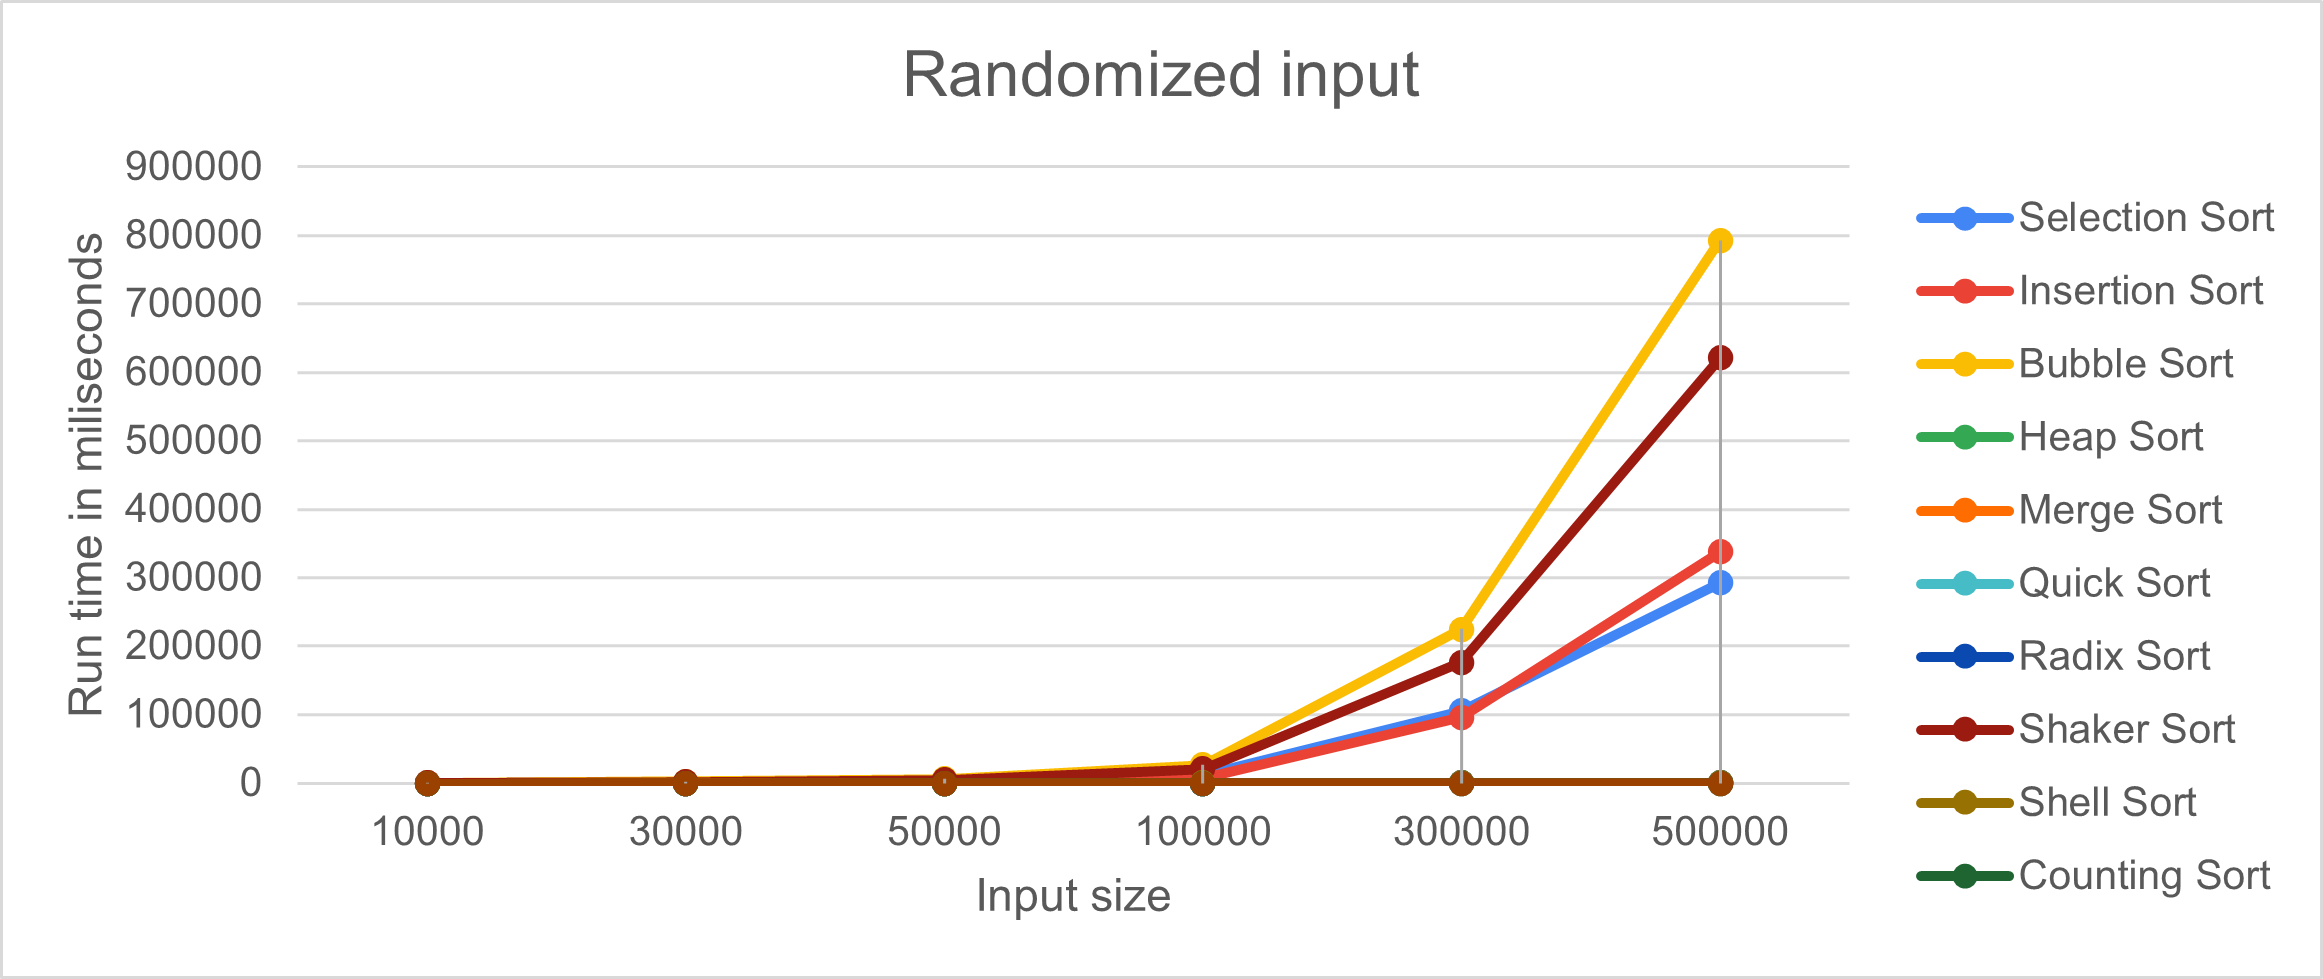
\includegraphics[scale = 0.8]{RandomLines.png}
\caption{ A line graph for visualizing the algorithms’ running times on random data.}
\centering
\end{figure}

\tab The same trend from figure 5 can be seen here with a slight deviation as merge sort takes a longer amount of time than selection sort. We can't explain this change in order, it may due to the randomized nature of the array. Because we've only run through two passes so there will be some differences compared to running a lot of passes.

\begin{figure}[H]
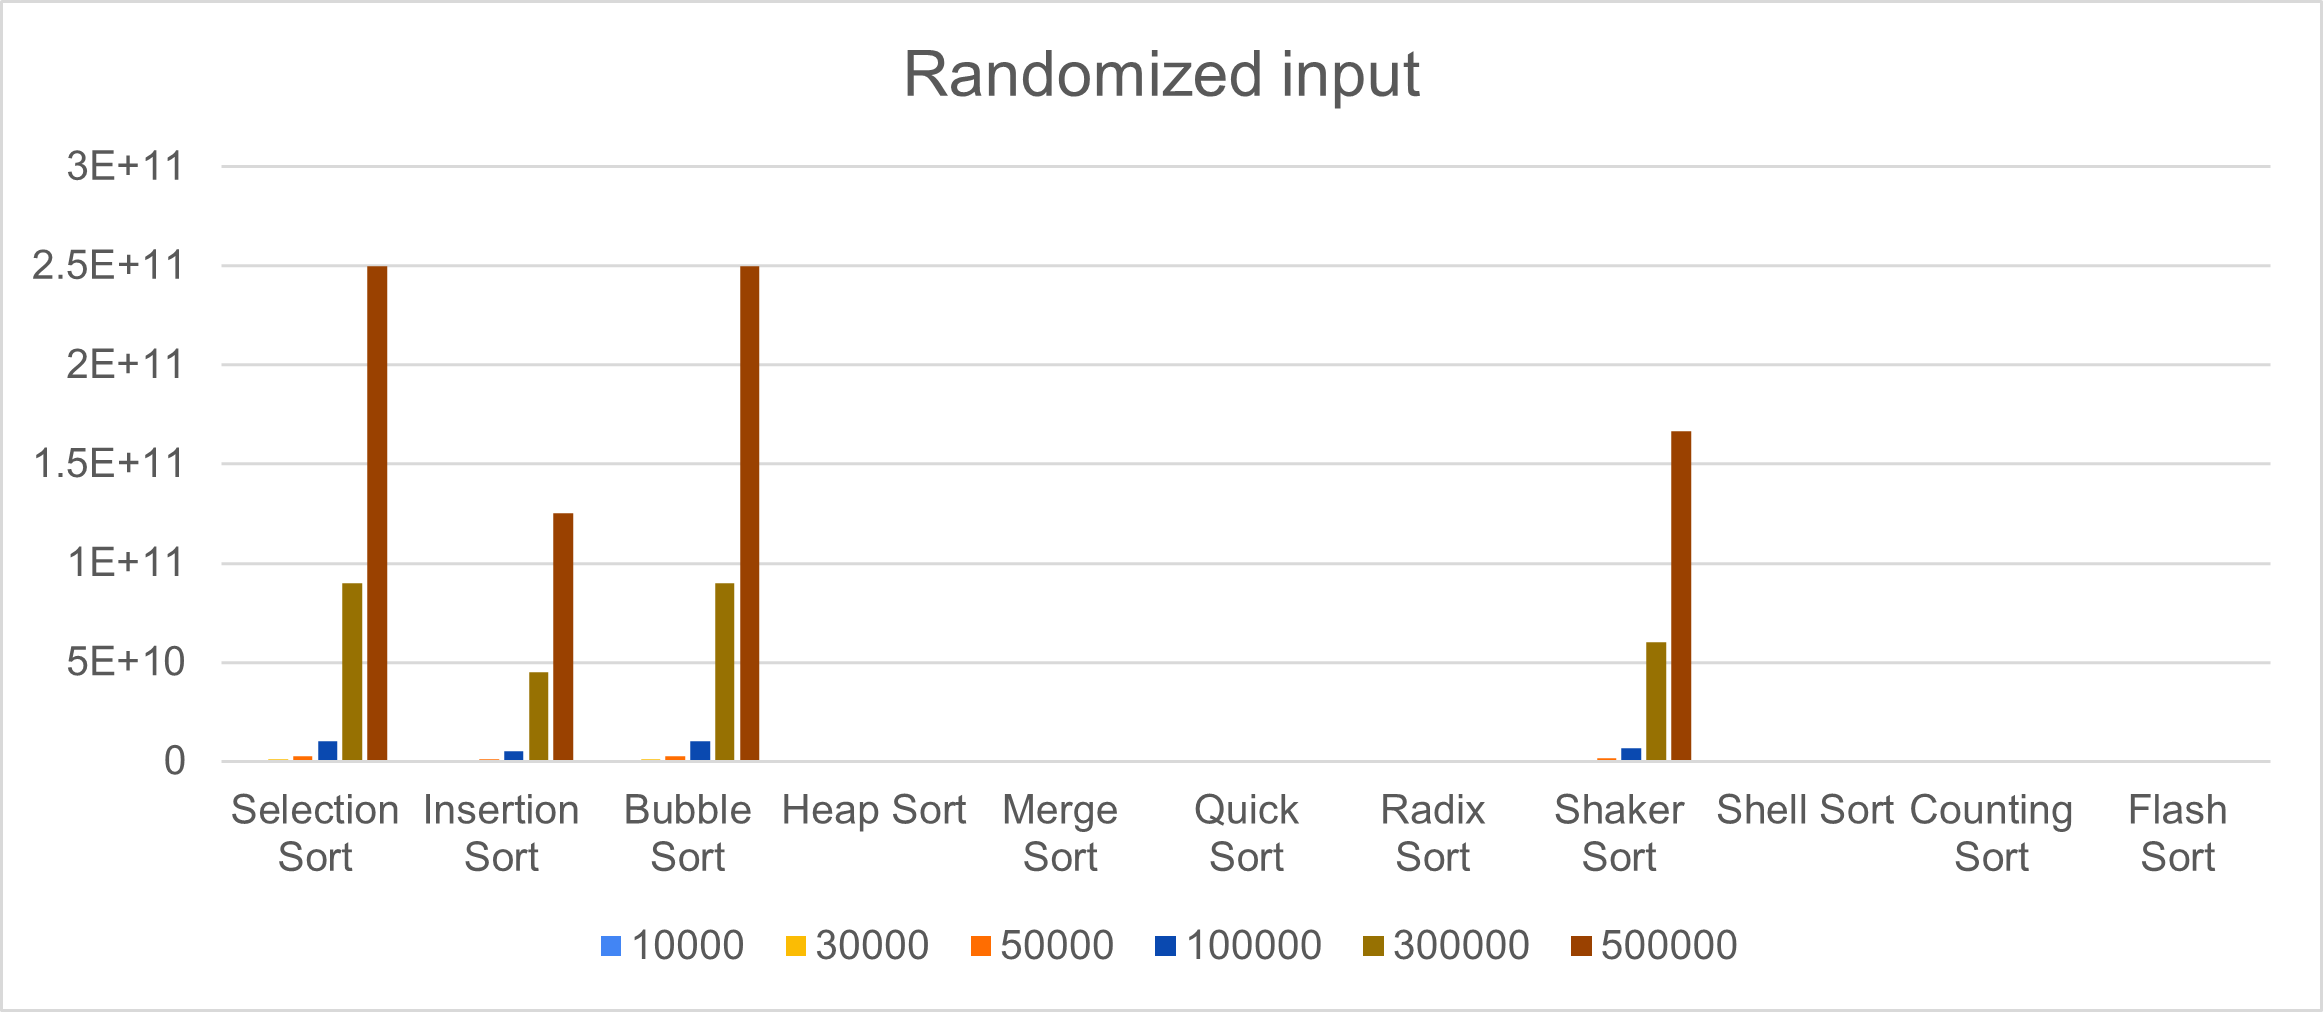
\includegraphics[scale = 0.8]{RandomBar.png}
\caption{A bar graph for visualizing the algorithms’ comparisons on sorted data.}
\centering
\end{figure}

Shaker and insertion sort number of comparisons have now reduced by quite a significant amount of time. This turnaround is because the data order is now randomized.

\pagebreak

\subsection{Comments}
Overall, from all four data orders, counting sort and flash sort both is the fastest sorting algorithm based on running time and comparisons. With bubble sort being the slowest\\
Stable sorting algorithms:
\begin{itemize}
    \item Insertion sort
    \item Bubble sort
    \item Merge sort
    \item Radix sort
    \item Counting sort
\end{itemize}
Unstable sorting algorithms:
\begin{itemize}
    \item Selection sort
    \item Heap sort
    \item Quick sort
    \item Shaker sort
    \item Shell sort
    \item Flash sort
\end{itemize}


\bigskip

\pagebreak



\section{Project organization and Programming notes}

\subsection{Project organization}
Library used (Allowed library for course):\\
\begin{itemize}
    \item We use time.h to measure the time instead of chrono.h
    \item fstream is used for file input and ouput
    \item iomanip is for setprecision()
    \item string and cstring both for string data type manipulation
    \item iostream for outputing to the console
\end{itemize}

Main file and subordinates:
\begin{itemize}
    \item DataGenerator.cpp: Data generation supplied by Mr. Bui Huy Thong
    \item header.h: Used to store all of our headers
    \item main.cpp: The program main source code
    \item Hai 21127267.cpp: Merge(), quick(), heap(), flash(), shaker() and shell() sort functions
    \item Nhan 21127382.cpp: Swap(), bubble(), insertion(), selection() sort functions
    \item Tri 21127556.cpp: The heart of our program, contains, file in out operations, printing to screen and measuring time and comparisons
\end{itemize}
\subsection{Programming notes}

\tab We've included a -help function to show all functions of the program for ease of use!\\
\tab This source code should be compiled in Visual Studio 2019 on Windows 10 for compatibily reasons.

\pagebreak



\section{References}

\href{https://en.wikipedia.org/wiki/Selection_sort#Complexity}{Information on Selection Sort}\\
\href{https://en.wikipedia.org/wiki/Selection_sort#Complexity}{Selection Sort complexity}\\
\href{https://cs.stackexchange.com/questions/111243/complexity-of-double-selection-sort}{Double Selection Sort complexity}
\href{https://www.geeksforgeeks.org/shellsort/}{Information of Shell Sort}\\
\href{https://en.wikipedia.org/wiki/Shellsort#Description}{Ideas of Shell Sort}\\
\href{https://stackabuse.com/bubble-sort-and-cocktail-shaker-sort-in-javascript/}{Buble Sort and Shaker Sort complexity}\\
\href{https://www.researchgate.net/publication/225806123_A_tight_lower_bound_for_the_worst_case_of_Bottom-Up-Heapsort}{More on bottom up heapsort time complexity}\\
\href{https://www.geeksforgeeks.org/heap-sort/}{Information of heap sort}\\
\href{https://cs.stackexchange.com/questions/11415/how-to-perform-bottom-up-construction-of-heaps}{Idea of Bottom Up Heap Sort}\\
\href{https://www.happycoders.eu/algorithms/heapsort/#Bottom-Up_Heapsort}{Information of Bottom Up Heap Sort}\\
\href{https://en.wikipedia.org/wiki/Binary_tree#Types_of_binary_trees}{Binary Tree}\\
\href{https://www.happycoders.eu/algorithms/heapsort/#Heapsort_Time_Complexity}{Heap Sort complexity}\\
\href{https://en.wikipedia.org/wiki/Heapsort#Variations}{Heap Sort Variants}\\
\href{https://www.geeksforgeeks.org/time-complexities-of-all-sorting-algorithms/}{Time and space complexity for all sorting algorithms and replacing best and worst notation with theta and omega respectively}\\
\href{https://en.wikipedia.org/wiki/Cocktail_shaker_sort#Complexity}{Explanation for line graph of reversed sorted data}\\
\href{https://www.geeksforgeeks.org/quick-sort/}{Information of Quick Sort}\\
\href{https://en.wikipedia.org/wiki/Quicksort#Variants}{Variants of Quick Sort}\\
\href{https://www.geeksforgeeks.org/radix-sort/}{Information of Radix Sort}\\
\href{https://www.simplilearn.com/tutorials/data-structure-tutorial/radix-sort#performance_of_radix_sort_algorithm}{Heap Sort complexity}\\
\href{https://www.growingwiththeweb.com/sorting/radix-sort-lsd/}{Variants of Radix Sort}\\
\href{https://www.javatpoint.com/shell-sort}{Information of Shell Sort}\\
\href{https://en.wikipedia.org/wiki/Counting_sort#Variant_algorithms}{Variants of Counting Sort}\\

\bigskip
\bigskip
\bigskip

\centerline{\Large{We appreciate your reading!}}

\end{document}